% ===============================
% Conception (inclut Identité Visuelle)
% ===============================

\section*{Introduction}
\addcontentsline{toc}{section}{Introduction}
Ce chapitre présente la démarche de conception de SayNote, en détaillant la méthodologie de planification, la conception UX, la modélisation, ainsi que l'identité visuelle de la marque. L'objectif est d'expliquer comment les choix de conception soutiennent la vision, l'expérience utilisateur et la cohérence de la marque.

% ===============================
% Section 1: Planification et UX
% ===============================
\section{Planification et conception UX}
% SayNote - Chapitre II: Planification et Conception UX
% Ce chapitre présente la planification du projet et la conception de l'expérience utilisateur


    
    \subsection{Planification du projet}
    
    \subsubsection{Méthodologie de planification}
    
    Pour le développement de SayNote, nous avons adopté une approche agile, plus précisément la méthodologie Scrum, complétée par des éléments de Design Thinking pour la conception UX. Cette combinaison nous permet d'itérer rapidement tout en gardant l'utilisateur au centre de notre processus de conception.
    
    \paragraph{Approche Agile Scrum}
    
    L'approche Scrum a été choisie pour sa flexibilité et sa capacité à s'adapter aux changements inhérents au développement d'un produit innovant comme SayNote. Nous avons organisé notre travail en sprints de deux semaines, chacun comportant les événements standards de Scrum:
    
    \begin{itemize}
        \item \textbf{Sprint Planning:} Au début de chaque sprint, l'équipe sélectionne les tâches du Product Backlog à réaliser, en se basant sur leur priorité et la capacité de l'équipe.
        
        \item \textbf{Daily Stand-up:} Réunions quotidiennes de 15 minutes pour synchroniser les activités et identifier les obstacles.
        
        \item \textbf{Sprint Review:} À la fin de chaque sprint, l'équipe présente les fonctionnalités développées aux parties prenantes pour obtenir des retours.
        
        \item \textbf{Sprint Retrospective:} L'équipe analyse ce qui a bien fonctionné et ce qui peut être amélioré pour le prochain sprint.
    \end{itemize}
    
    Cette approche nous permet de livrer régulièrement des incréments de produit fonctionnels et d'ajuster notre direction en fonction des retours utilisateurs et des défis techniques rencontrés.
    
    \paragraph{Design Thinking pour l'UX}
    
    En parallèle de Scrum, nous avons intégré le processus de Design Thinking pour la conception de l'expérience utilisateur, qui comprend cinq phases:
    
    \begin{enumerate}
        \item \textbf{Empathie:} Comprendre profondément les besoins, les frustrations et les aspirations des utilisateurs potentiels à travers des entretiens et des observations.
        
        \item \textbf{Définition:} Synthétiser les connaissances acquises pour définir clairement les problèmes à résoudre.
        
        \item \textbf{Idéation:} Générer un large éventail d'idées et de solutions potentielles sans contraintes initiales.
        
        \item \textbf{Prototypage:} Créer des représentations tangibles des solutions les plus prometteuses.
        
        \item \textbf{Test:} Recueillir les retours des utilisateurs sur les prototypes pour affiner et améliorer les solutions.
    \end{enumerate}
    
    Cette approche centrée sur l'utilisateur est particulièrement pertinente pour SayNote, où l'interaction vocale nécessite une compréhension fine des attentes et des comportements des utilisateurs.
    
        
    \subsubsection{Planification}
    
    \paragraph{Roadmap du projet}
    
    La roadmap de SayNote a été structurée en quatre phases principales, chacune comportant plusieurs sprints:
    
    \begin{enumerate}
        \item \textbf{Phase de recherche et de conception (2 mois):}
        \begin{itemize}
            \item Recherche utilisateur et analyse concurrentielle
            \item Définition des personas et des scénarios d'utilisation
            \item Conception de l'architecture du système
            \item Wireframing et prototypage initial
        \end{itemize}
        
        \item \textbf{Phase de développement MVP (4 mois):}
        \begin{itemize}
            \item Mise en place de l'infrastructure technique
            \item Développement du backend et de l'API
            \item Implémentation de l'éditeur de notes par blocs (avec BlockNote.js)
            \item Intégration de la reconnaissance vocale de base
            \item Développement de l'interface utilisateur mobile (Expo/React Native)
        \end{itemize}
        
        \item \textbf{Phase d'amélioration et d'expansion (3 mois):}
        \begin{itemize}
            \item Optimisation des algorithmes de traitement du langage naturel
            \item Expansion des commandes vocales supportées
            \item Développement de l'interface web
            \item Implémentation des fonctionnalités de sous-pages et de hiérarchie de notes
        \end{itemize}
        
        \item \textbf{Phase de finalisation et de lancement (1 mois):}
        \begin{itemize}
            \item Tests utilisateurs approfondis
            \item Correction des bugs et optimisations finales
            \item Préparation du matériel marketing
            \item Lancement officiel de l'application
        \end{itemize}
    \end{enumerate}
    
    % Explication brève avant chaque figure
        \begin{figure}[htbp]
        \centering
        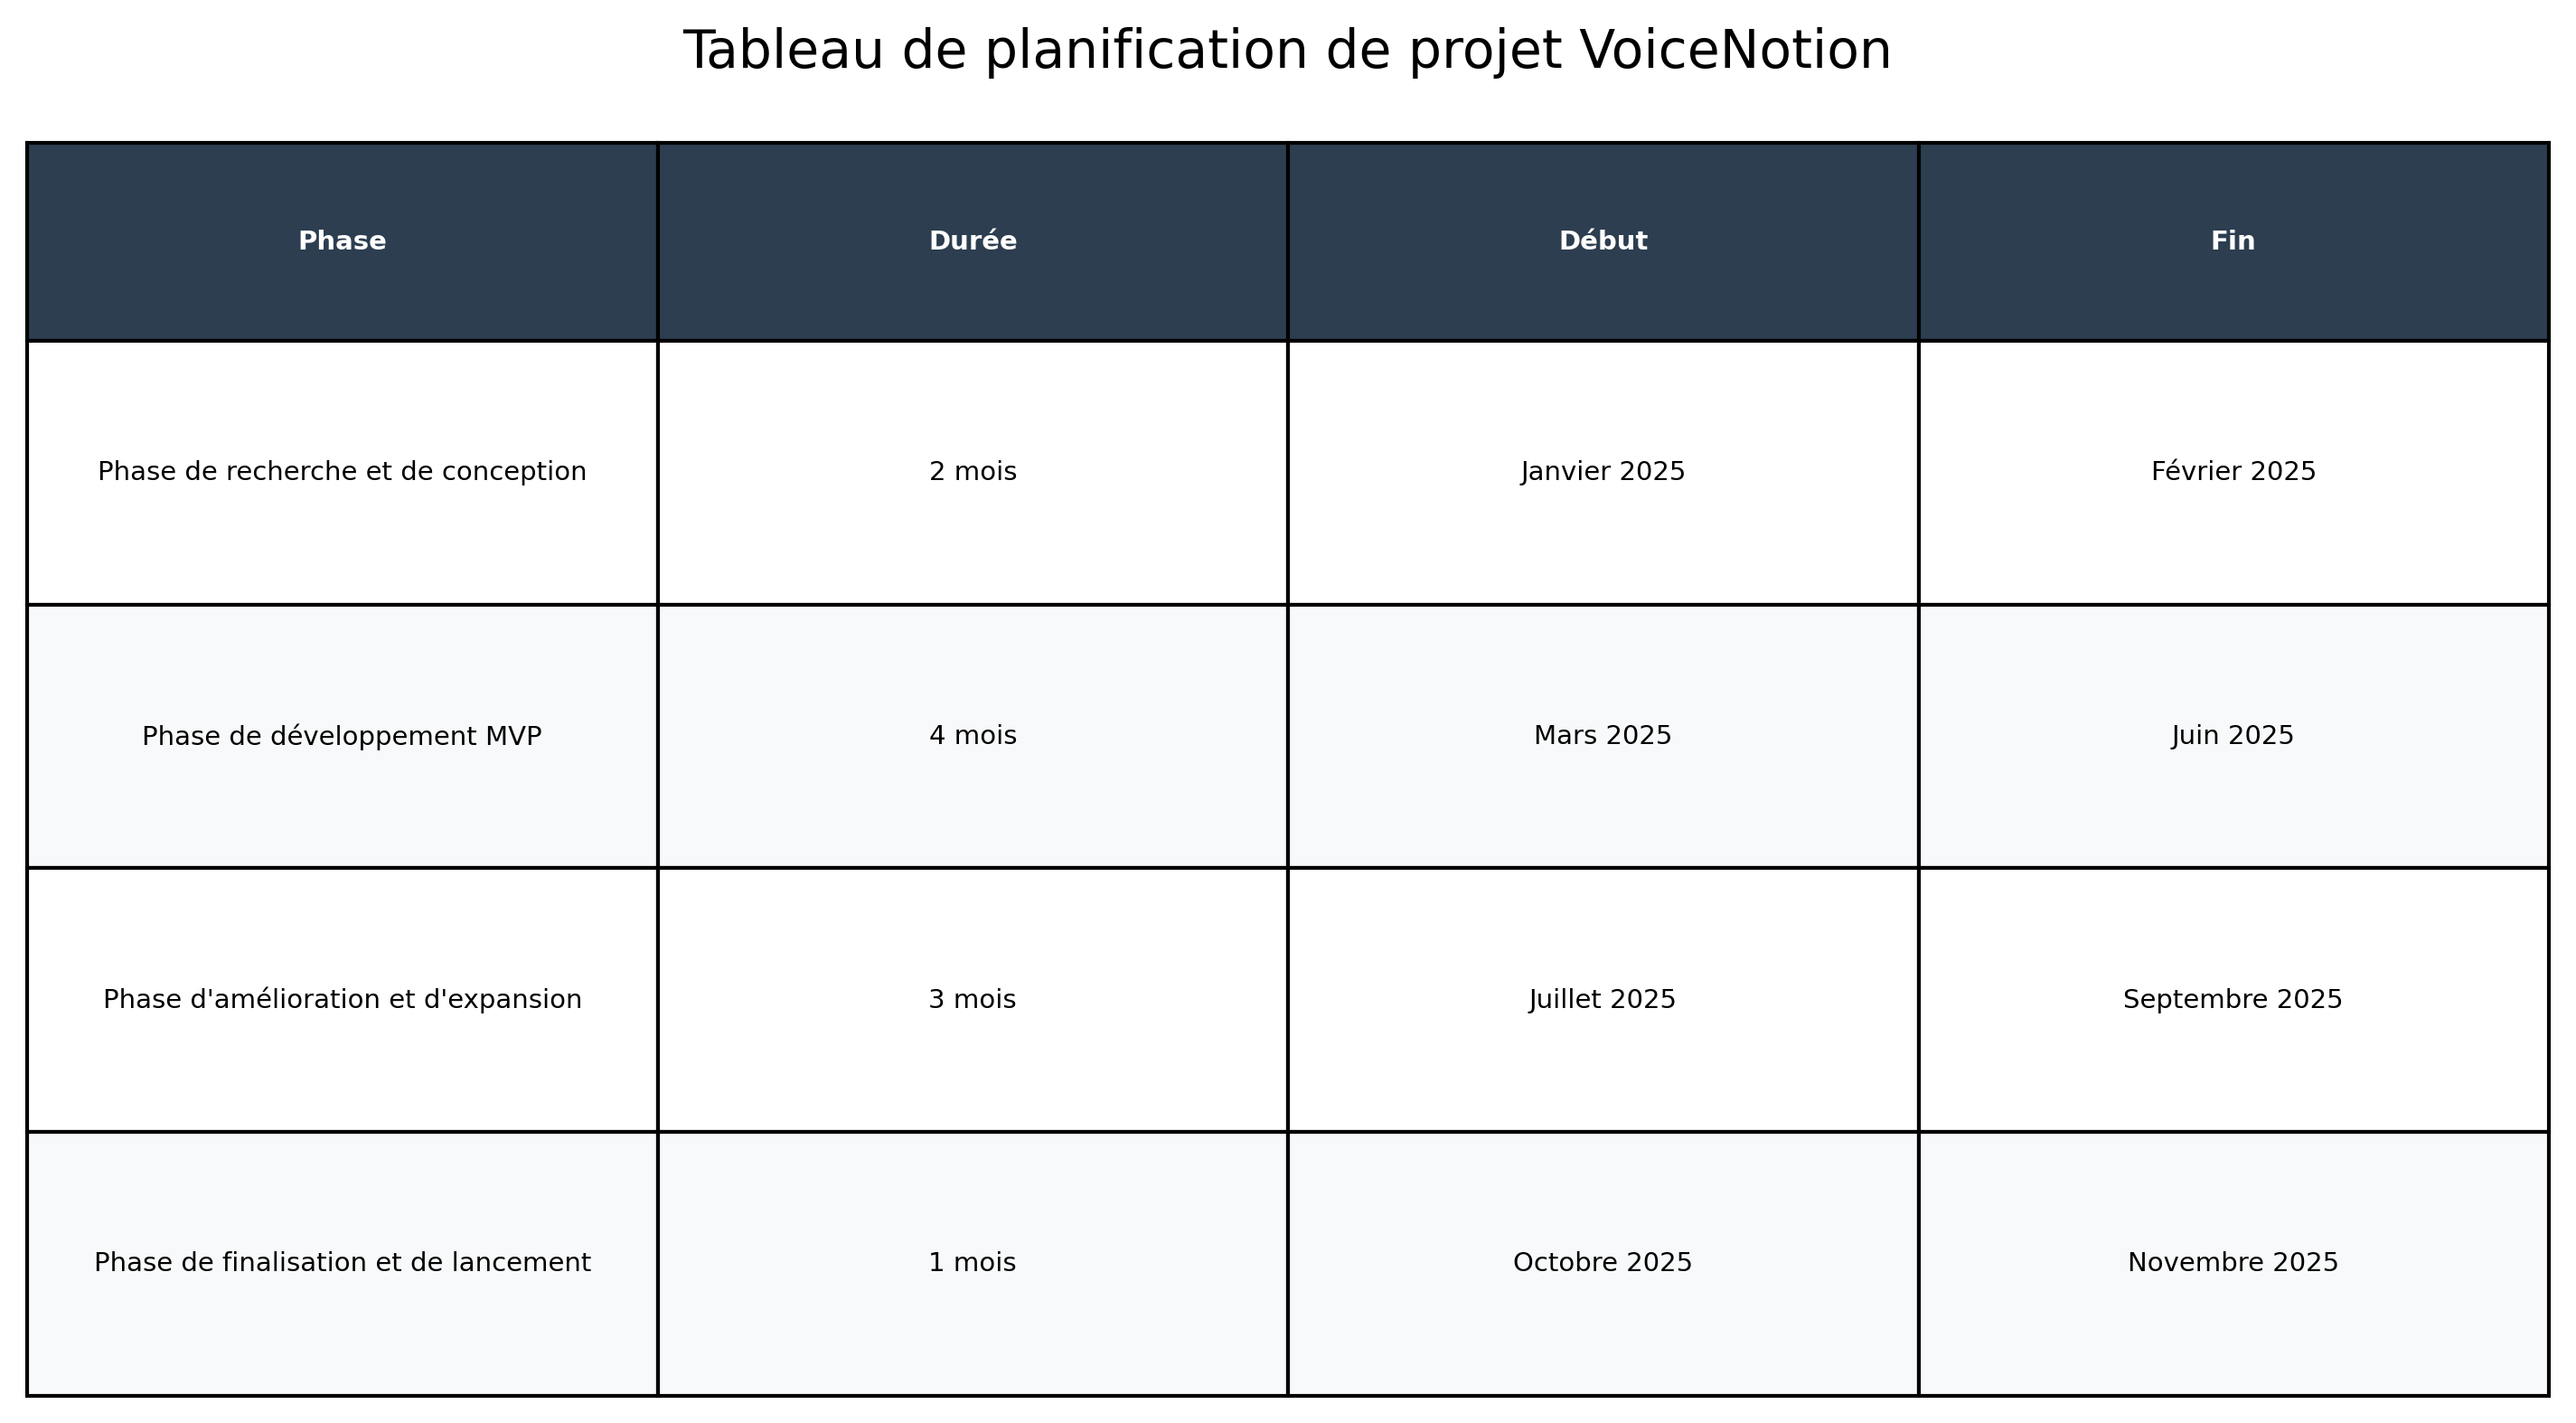
\includegraphics[width=0.9\textwidth]{assets/docs/planification_table.png}
        \caption{Tableau de planification de projet}
        \label{fig:planification_table}
    \end{figure}
    
    % Explication brève avant chaque figure
        \begin{figure}[htbp]
        \centering
        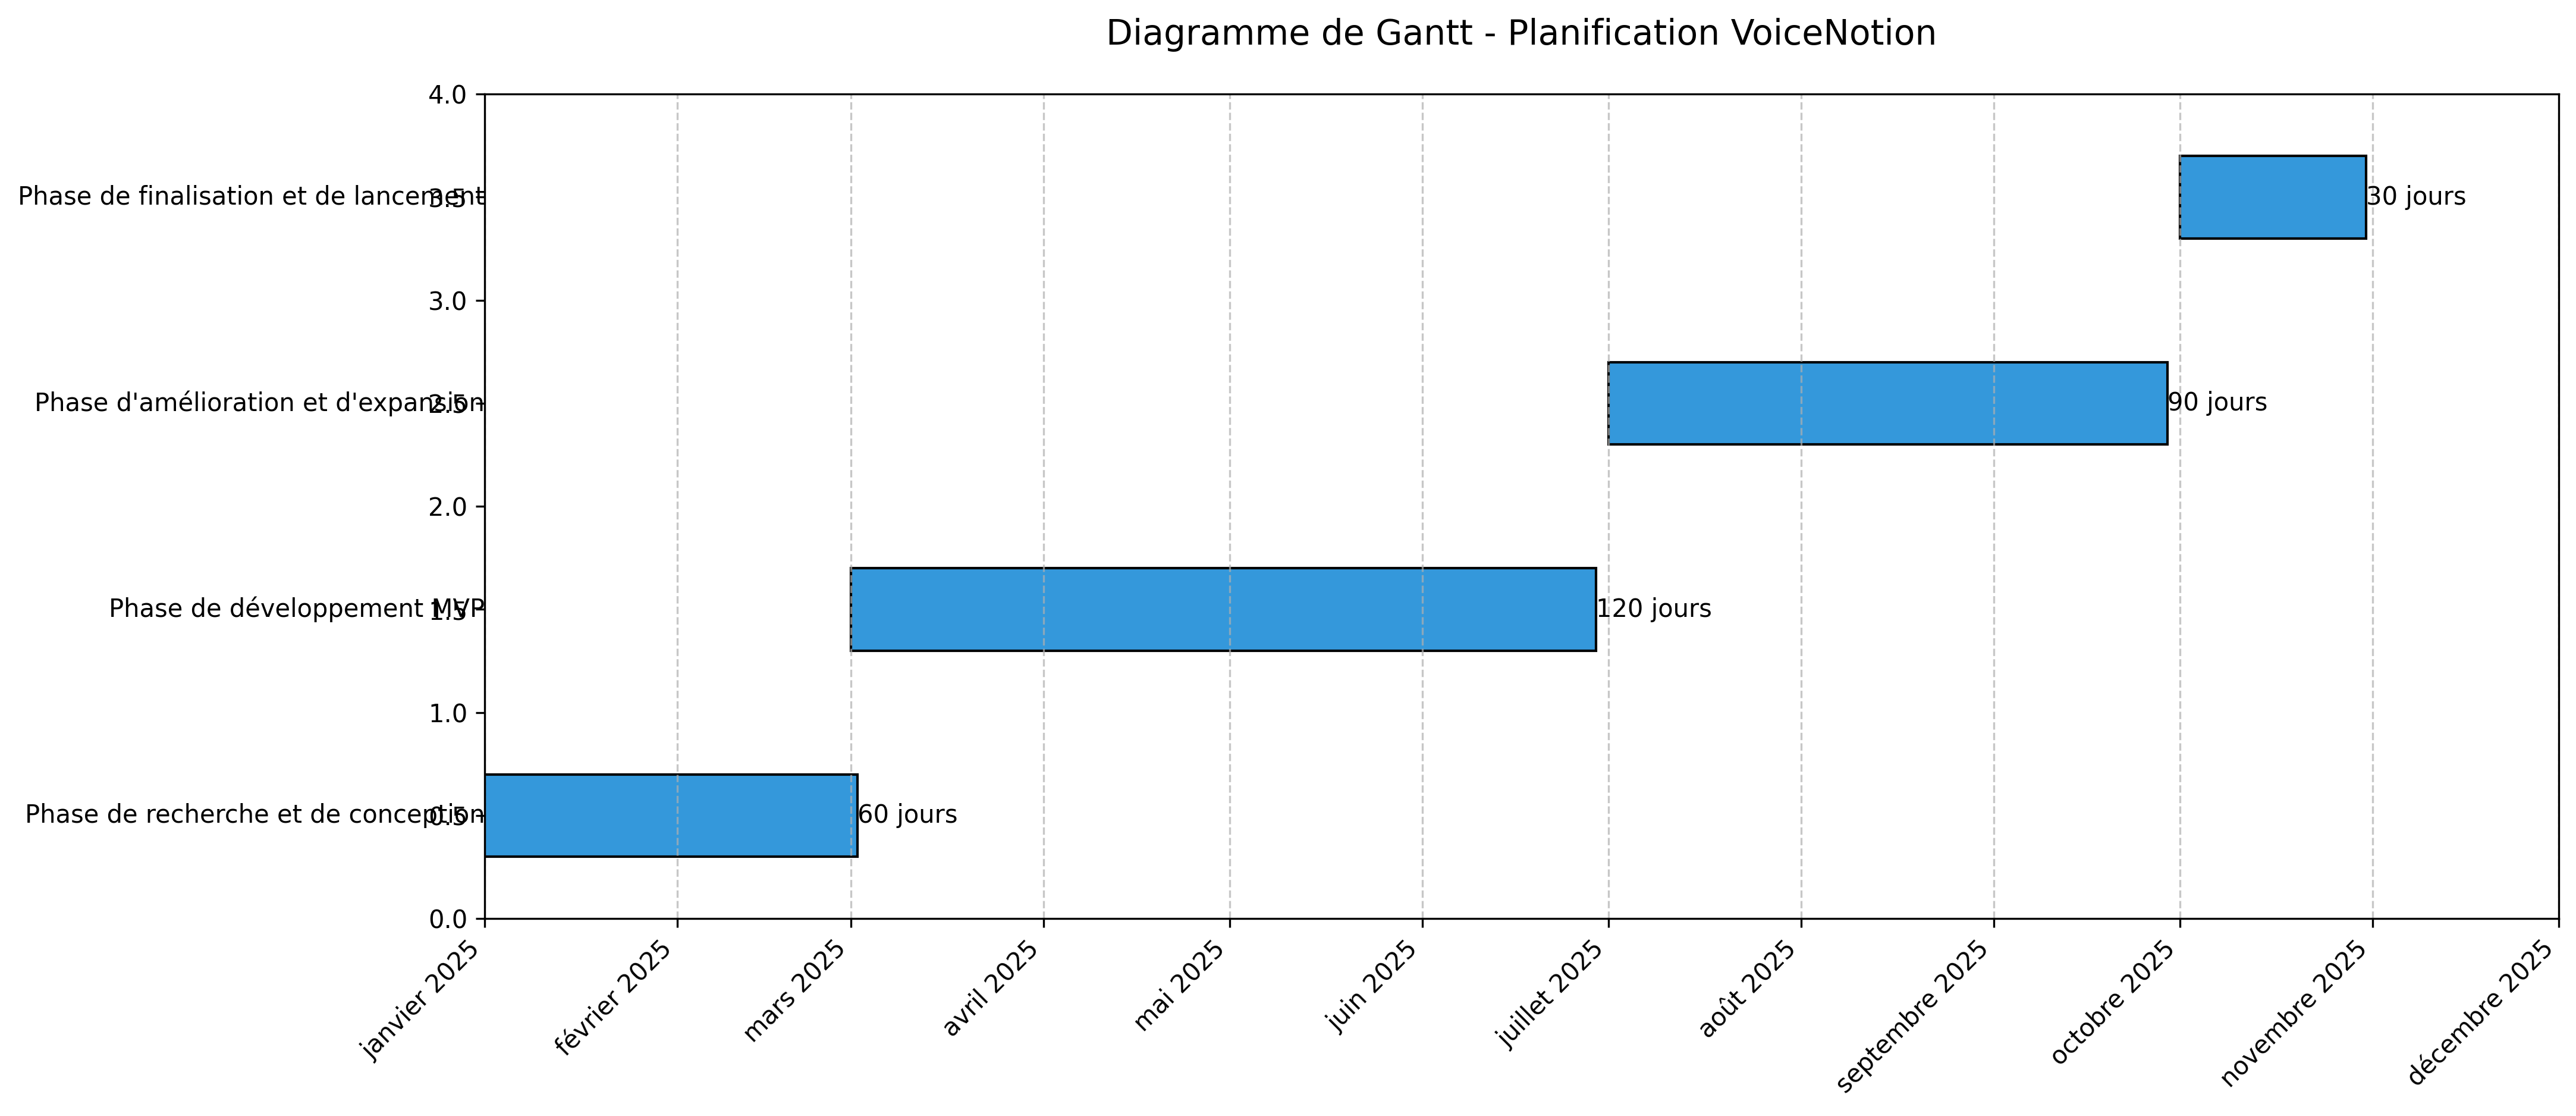
\includegraphics[width=0.9\textwidth]{assets/docs/gantt_chart.png}
        \caption{Diagramme de Gantt de planification de projet}
        \label{fig:gantt_chart}
    \end{figure}
    
    \paragraph{Calendrier détaillé (avril–juin 2025)}
Le tableau~\ref{fig:planification_table} fournit un aperçu visuel ; ci-dessous figure le même planning avec les dates exactes :

\begin{itemize}
  \item \textbf{Recherche \& planification} : 01/04/2025 – 07/04/2025
  \item \textbf{Conception graphique} : 08/04/2025 – 22/04/2025
    \begin{itemize}
      \item \textit{UI/UX Design} : 23/04/2025 – 30/04/2025
      \item \textit{Design System} : 23/04/2025 – 25/04/2025
      \item \textit{Prototypage} : 26/04/2025 – 28/04/2025
      \item \textit{Wireframing} : 29/04/2025 – 30/04/2025
      \item \textit{Animation vidéo} : 01/05/2025 – 03/05/2025
    \end{itemize}
  \item \textbf{Architecture système} : 04/05/2025 – 07/05/2025
    \begin{itemize}
      \item \textit{Conception base de données} : 08/05/2025 – 10/05/2025
    \end{itemize}
  \item \textbf{Développement \& build} : 11/05/2025 – 10/06/2025
    \begin{itemize}
      \item \textit{API (Back-End)} : 11/05/2025 – 24/05/2025
      \item \textit{Site client (Web)} : 11/05/2025 – 31/05/2025
      \item \textit{Application mobile} : 11/05/2025 – 31/05/2025
      \item \textit{Hébergement \& déploiement} : 01/06/2025 – 05/06/2025
      \item \textit{Tests} : 06/06/2025 – 10/06/2025
    \end{itemize}
  \item \textbf{Synthèse et documentation} : 11/06/2025 – 20/06/2025
    \begin{itemize}
      \item \textit{Rapport de projet} : 13/06/2025 – 17/06/2025
      \item \textit{Présentation} : 18/06/2025 – 20/06/2025
    \end{itemize}
\end{itemize}

\paragraph{Gestion des risques}
    
    Nous avons identifié plusieurs risques potentiels pour le projet et élaboré des stratégies d'atténuation:
    
    \begin{table}[H]
    \centering
    \begin{tabular}{|p{3cm}|p{5cm}|p{5cm}|}
    \hline
    \textbf{Risque} & \textbf{Impact potentiel} & \textbf{Stratégie d'atténuation} \\
    \hline
    Précision limitée de la reconnaissance vocale & Frustration utilisateur, abandon de l'application & Implémentation d'un mécanisme de correction, modes d'entrée alternatifs, tests extensifs avec différents accents \\
    \hline
    Complexité technique de l'intégration BlockNote & Retards de développement, problèmes de performance & Spike techniques précoces, exploration des alternatives, recrutement d'expertise spécifique \\
    \hline
    Expérience utilisateur non intuitive & Courbe d'apprentissage abrupte, faible adoption & Tests utilisateurs fréquents, approche itérative, tutoriels intégrés \\
    \hline
    Limites des API Gemini & Fonctionnalités restreintes, dépendance à un tiers & Plan de secours avec solutions alternatives, découplage de l'architecture \\
    \hline
    Problèmes de performance sur appareils mobiles & Lenteur, consommation excessive de batterie & Optimisation continue, tests sur différents appareils, métriques de performance \\
    \hline
    \end{tabular}
    \caption{Tableau des risques et stratégies d'atténuation}
    \label{tab:risk_management}
    \end{table}
    
    \subsection{Expérience d'utilisateur (UX)}
    
    \subsubsection{Recherche}
    
    La conception de SayNote est fondée sur une recherche approfondie pour comprendre les besoins, les attentes et les points de friction des utilisateurs potentiels en matière de prise de notes.
    
    \paragraph{Méthodologie de recherche}
    
    Notre recherche a combiné plusieurs approches:
    
    \begin{itemize}
        \item \textbf{Entretiens qualitatifs:} Nous avons mené 15 entretiens approfondis avec des utilisateurs potentiels issus de nos groupes cibles (étudiants, professionnels, créateurs de contenu).
        
        \item \textbf{Analyse concurrentielle:} Étude détaillée des applications existantes (Notion, Evernote, OneNote, Google Keep) pour identifier les forces, les faiblesses et les opportunités d'innovation.
        
        \item \textbf{Sondage en ligne:} Un questionnaire distribué à 50 participants pour quantifier les préférences et les habitudes de prise de notes.
        
        \item \textbf{Sessions d'observation:} Observation de 8 utilisateurs dans leur environnement naturel pendant qu'ils prenaient des notes, révélant des comportements et des défis non exprimés lors des entretiens.
    \end{itemize}
    
    \paragraph{Principaux insights}
    
    Cette recherche a mis en lumière plusieurs insights clés qui ont guidé notre conception:
    
    \begin{enumerate}
        \item 78\% des participants trouvent que la saisie manuelle limite leur capacité à capturer rapidement les informations lors de réunions ou de conférences.
        
        \item Les utilisateurs de Notion apprécient la flexibilité de la structure par blocs, mais 65\% trouvent la courbe d'apprentissage trop abrupte.
        
        \item 92\% des participants ont exprimé de l'intérêt pour les commandes vocales, mais 71\% craignent qu'elles ne soient pas assez précises ou intuitives.
        
        \item Les utilisateurs mobiles (81\% de notre échantillon) prennent des notes dans des contextes variés où le clavier n'est pas toujours optimal (transports, déplacements, exercice).
        
        \item La structuration post-capture est identifiée comme l'un des plus grands défis, avec 85\% des participants qui admettent ne jamais réorganiser leurs notes brutes par manque de temps.
    \end{enumerate}
    
    % Explication brève avant chaque figure
        \begin{figure}[htbp]
        \centering
        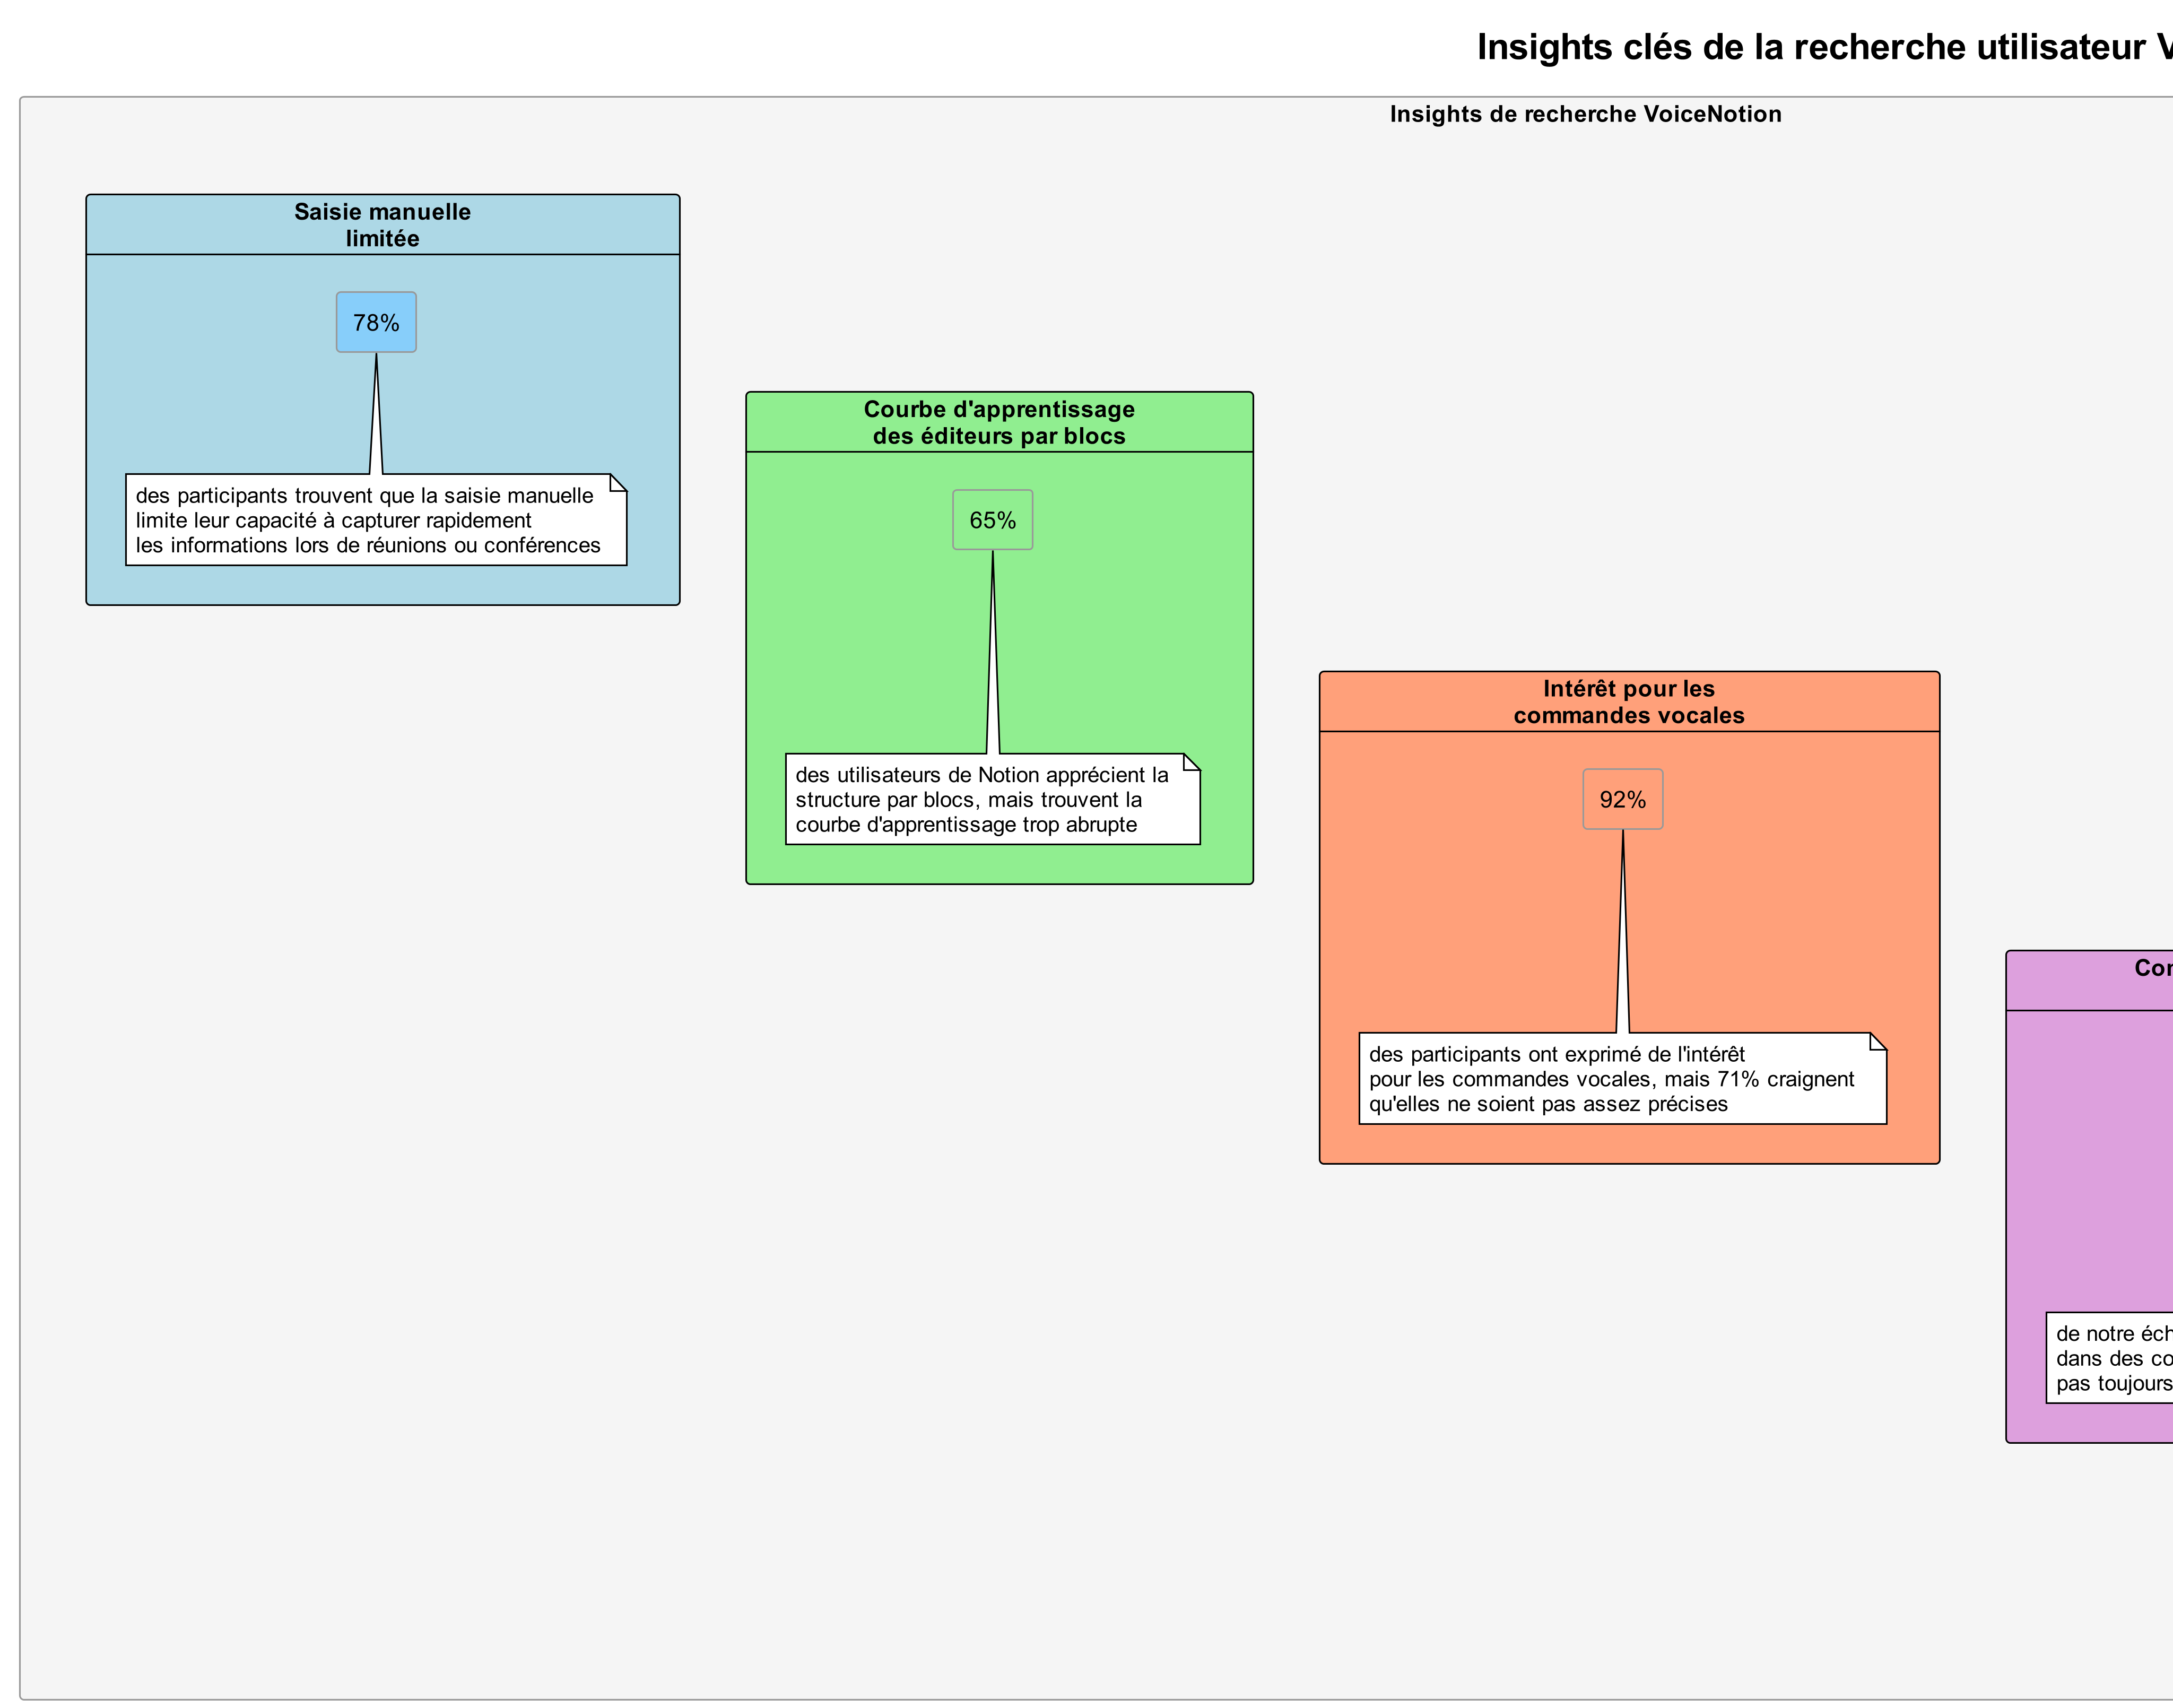
\includegraphics[width=0.75\textwidth]{assets/docs/user_research_insights.png}
        \caption{Synthèse des principaux insights de recherche utilisateur}
        \label{fig:user_research_insights}
    \end{figure}
    
    \subsubsection{Empathie}
    
    \paragraph{Personas utilisateur}
    
    Basés sur notre recherche, nous avons développé deux personas principaux qui représentent nos utilisateurs cibles:
    
    \begin{figure}[H]
        \centering
        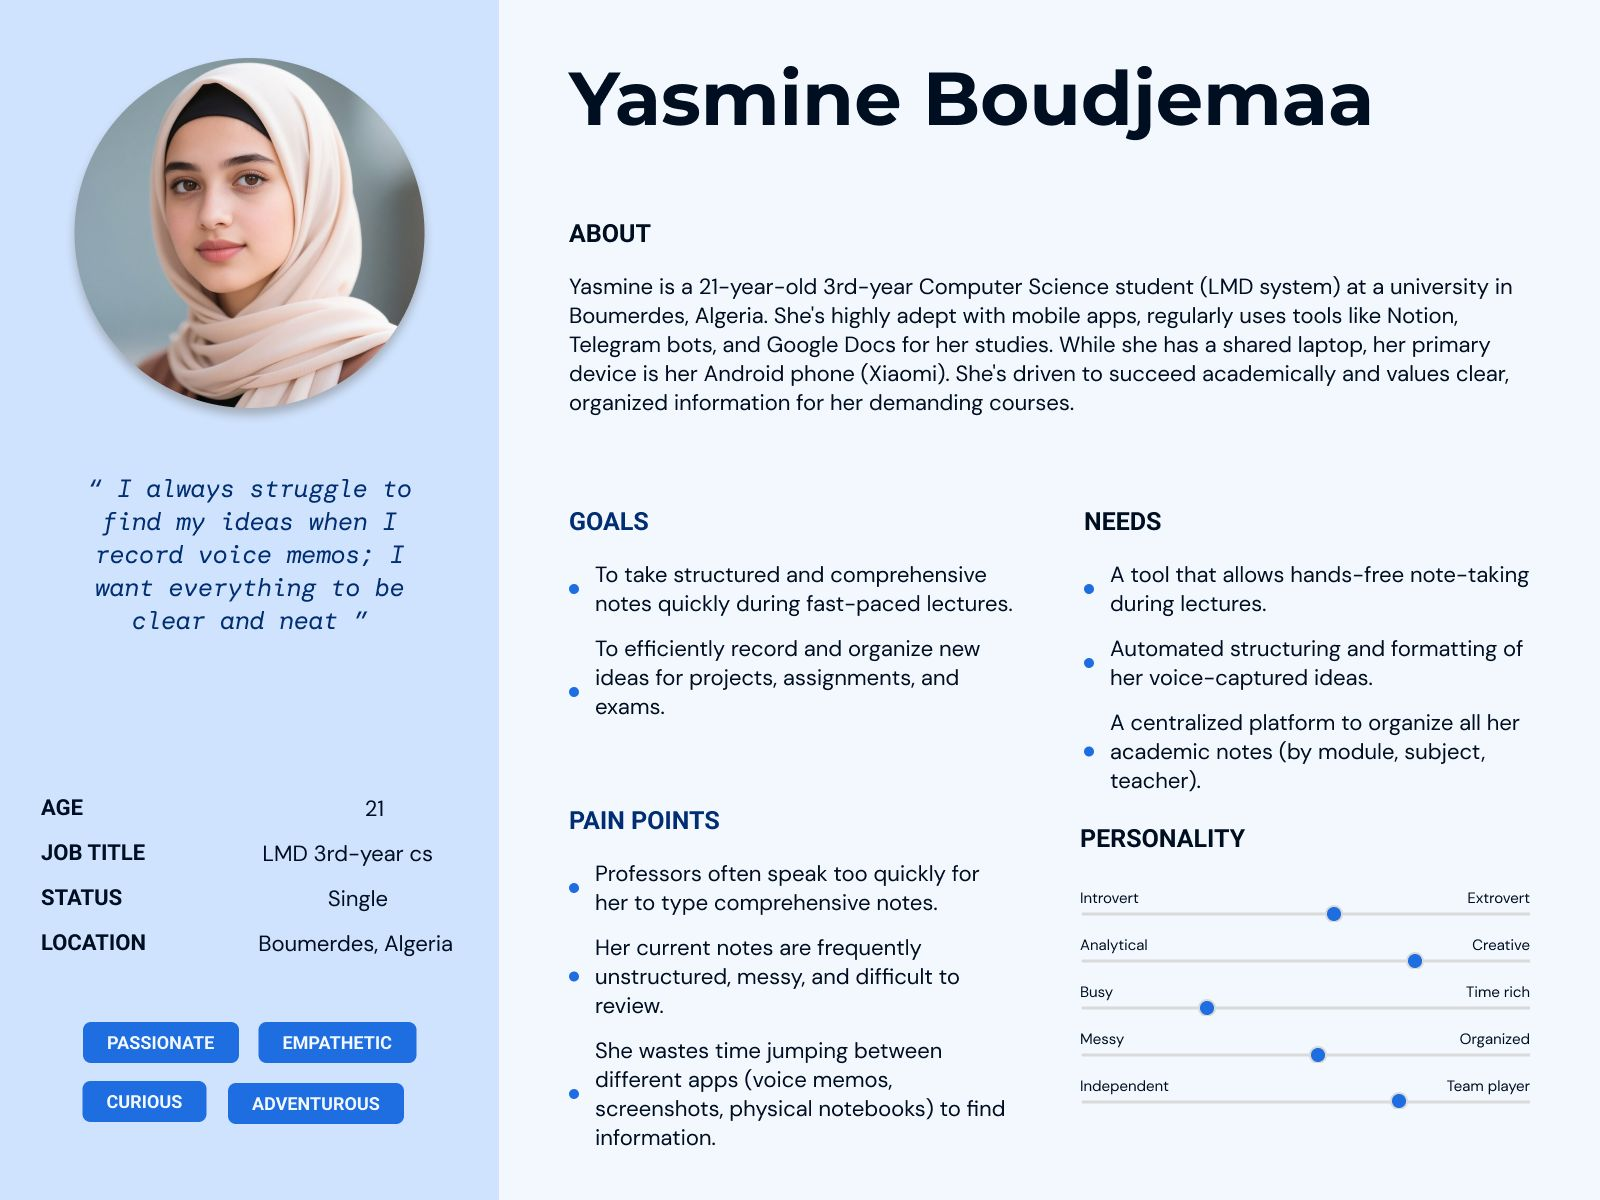
\includegraphics[width=\textwidth]{assets/docs/yassmine-personaa.jpg}
    \end{figure}
    
    \paragraph{Persona 1: Yasmine l'Étudiante en Informatique}
    
    
    \begin{itemize}
        \item \textbf{Profil:} Étudiante de 21 ans en 3ème année d'Informatique à Boumerdes. Adepte des applications mobiles (Notion, Telegram, Google Docs), elle utilise principalement son téléphone Android.
        \item \textbf{Objectifs:} Prendre des notes structurées rapidement en cours, organiser efficacement ses idées, et maintenir un système de notes propre sans réécriture manuelle.
        \item \textbf{Frustrations:} Difficulté à suivre les professeurs qui parlent vite, notes désordonnées, perte de temps entre plusieurs applications, et réorganisation manuelle fastidieuse.
        \item \textbf{Comportements:} Jongle entre mémos vocaux, captures d'écran et cahiers. Passe beaucoup de temps à réécrire et à organiser ses notes, souvent tard le soir.
        \item \textbf{Citation:} "J'ai toujours du mal à retrouver mes idées lorsque j'enregistre des mémos vocaux ; je veux que tout soit clair et bien rangé."
    \end{itemize}

    \begin{figure}[H]
        \centering
        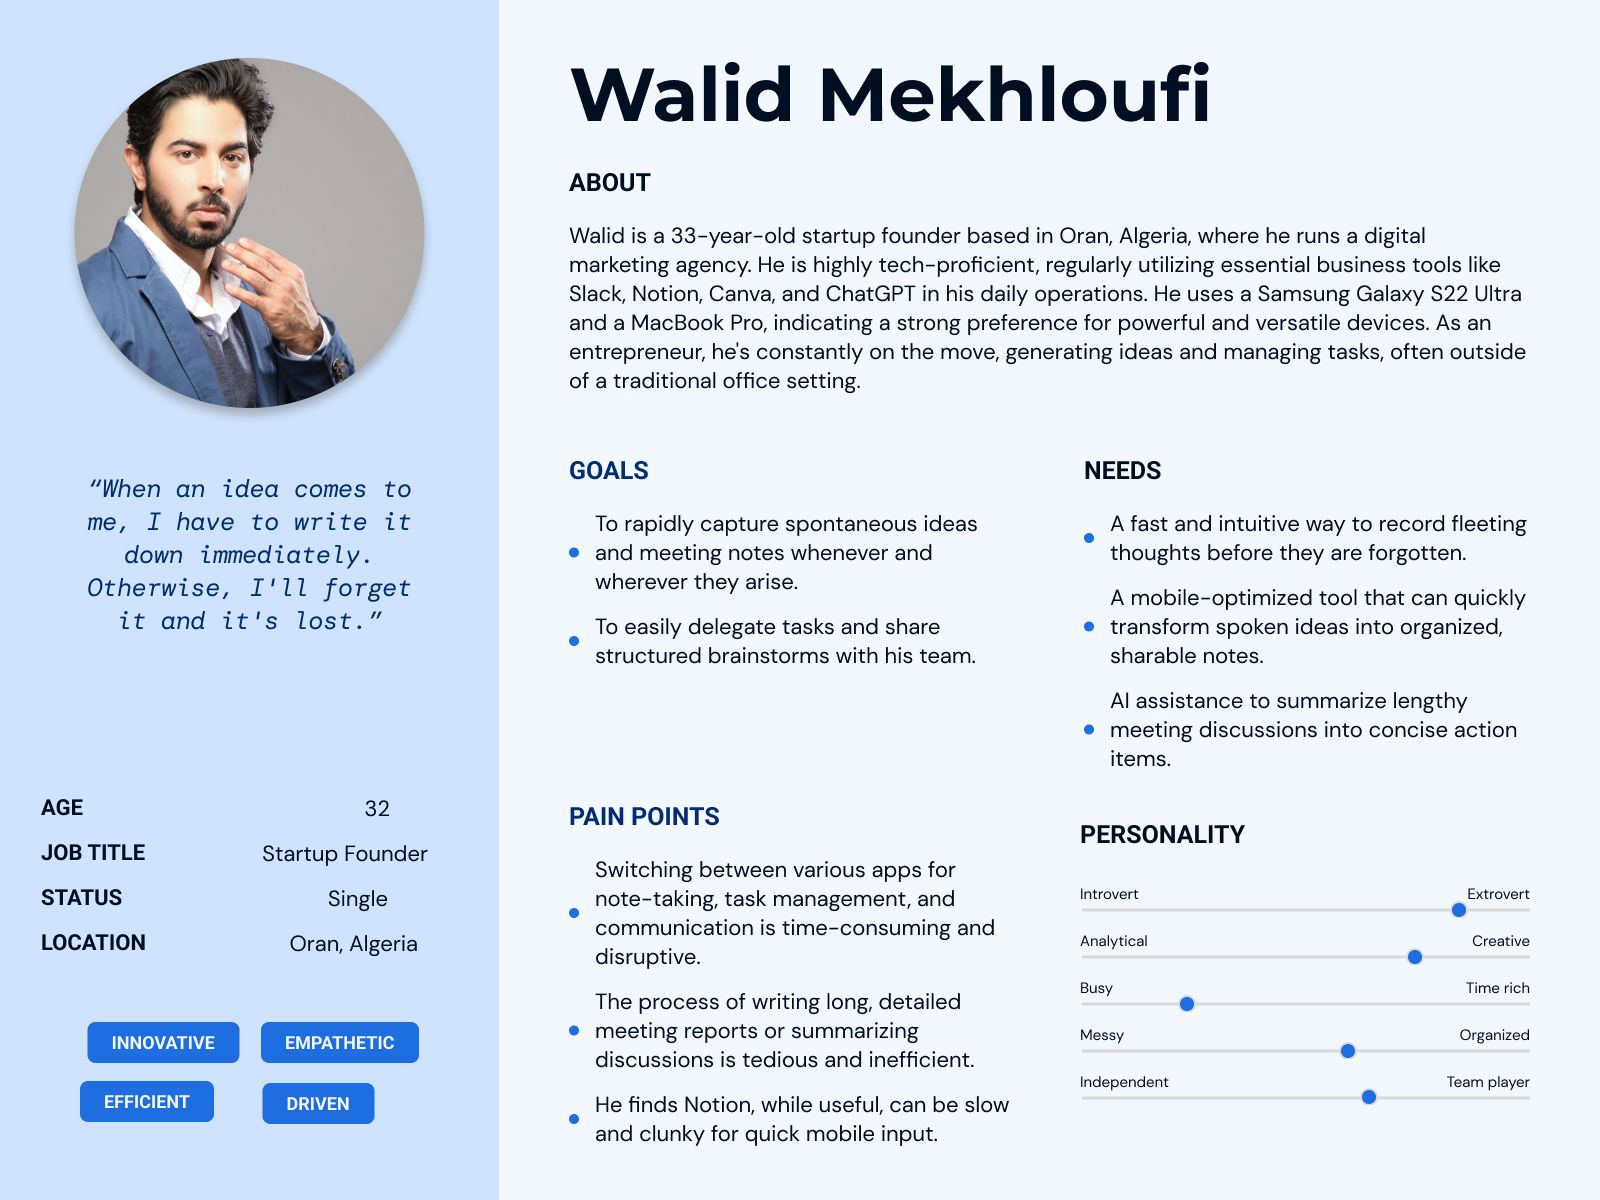
\includegraphics[width=\textwidth]{assets/docs/walid-persona.jpg}
    \end{figure}



    \paragraph{Persona 2: Walid l'Entrepreneur}

    \begin{itemize}
        \item \textbf{Profil:} Fondateur de startup de 33 ans (agence de marketing digital) à Oran. Il utilise des outils comme Slack, Notion, et ChatGPT sur son Samsung Galaxy S22 Ultra et MacBook Pro.
        \item \textbf{Objectifs:} Capturer rapidement les idées spontanées, déléguer facilement des tâches, et organiser ses idées et tâches par commandes vocales, notamment en déplacement.
        \item \textbf{Besoins:} Un moyen rapide pour enregistrer ses pensées, un outil mobile qui transforme la parole en notes structurées et partageables, et une IA pour résumer les réunions en actions concrètes.
        \item \textbf{Frustrations:} Oublie souvent des idées précieuses faute de pouvoir les noter instantanément, perd du temps à jongler entre les applications, et trouve la rédaction de comptes-rendus longue et inefficace.
        \item \textbf{Citation:} "Quand une idée me vient, je dois l’écrire direct. Sinon, je l’oublie et c’est mort."
    \end{itemize}
    
    
    % ===============================
    % Section: Wireframes et Design System
    % ===============================
    
    \subsubsection{Wireframes de l'application mobile}
    
    Avant le prototypage final, des wireframes basse fidélité ont été réalisés pour définir la structure et l'expérience utilisateur de l'application mobile SayNote.
    
    % Explication brève avant la figure
        \textit{La figure suivante présente un wireframe représentatif de l'application mobile.}
    \begin{figure}[H]
        \centering
        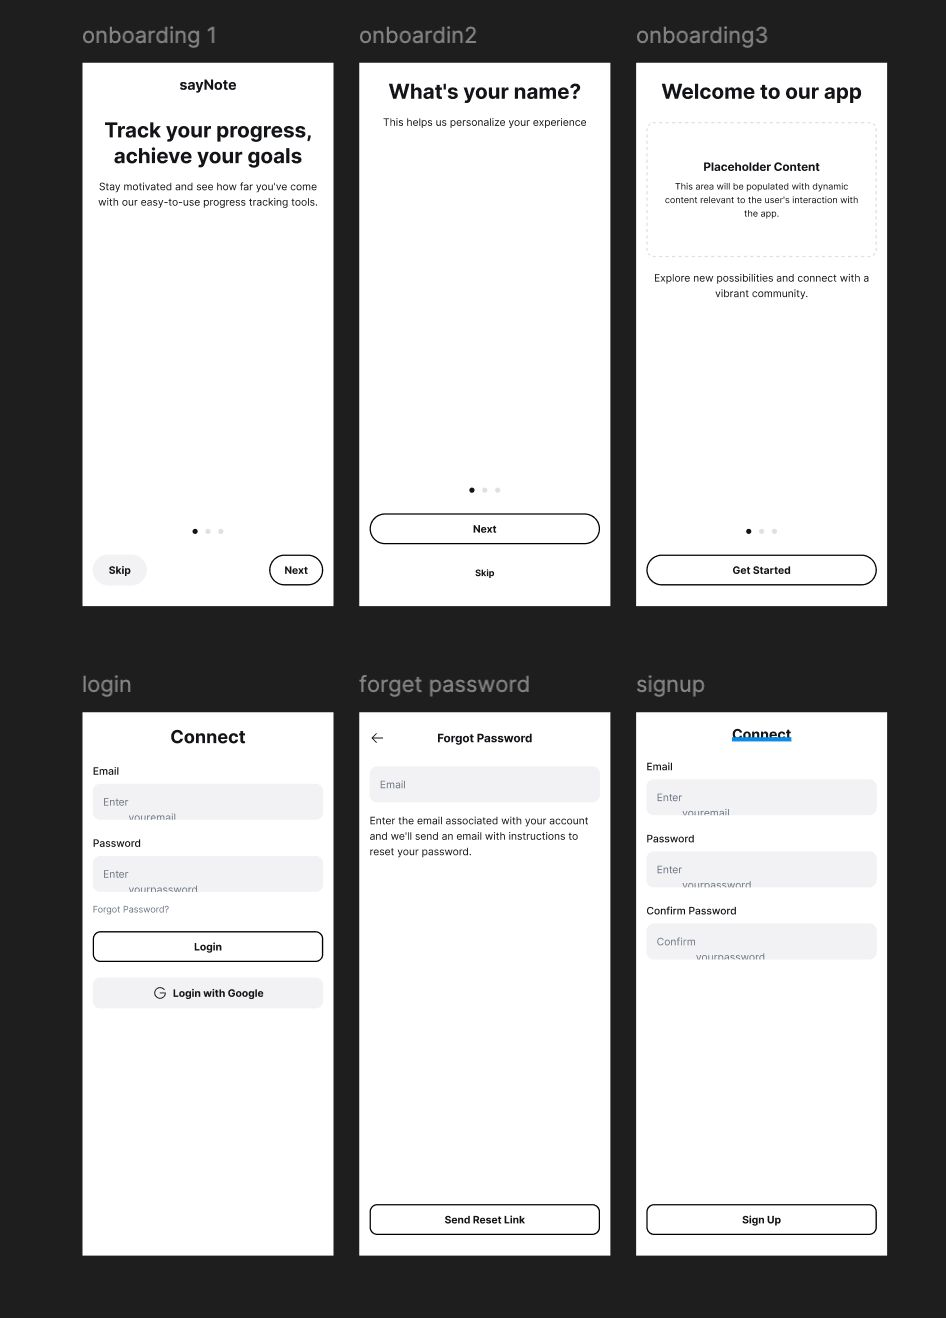
\includegraphics[width=0.9\textwidth]{assets/docs/mobile/wireframe_app-1.jpg}
        \caption{Wireframe de l'application mobile SayNote. \newline\textit{Ce schéma illustre la navigation et la disposition générale des écrans de authentification.}}
        \label{fig:wireframe_app_auth}
    \end{figure}
    
    \begin{figure}[H]
        \centering
        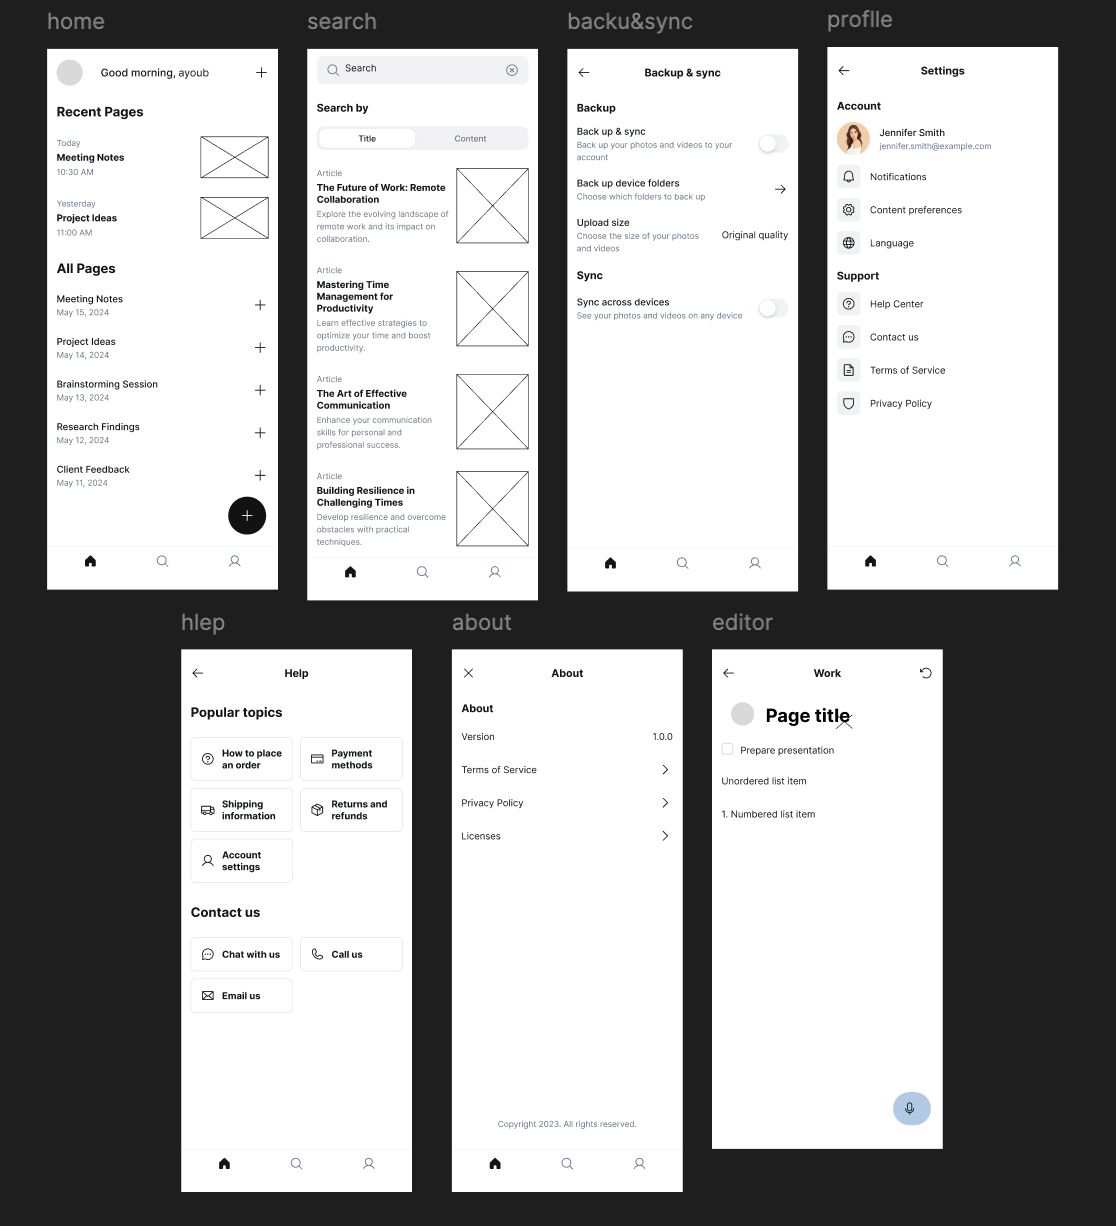
\includegraphics[width=0.9\textwidth]{assets/docs/mobile/wireframe_app-2.jpg}
        \caption{Wireframe de l'application mobile SayNote. \newline\textit{Ce schéma illustre la navigation et la disposition générale des écrans principaux.}}
        \label{fig:wireframe_app_main}
    \end{figure}
    
    
    \subsubsection{Synthèse du Design System}
    
    Une synthèse du design system a été réalisée pour garantir la cohérence visuelle et fonctionnelle de l'ensemble des interfaces.
    
        
    \paragraph{Scénarios d'utilisations}
    
    Pour chaque persona, nous avons développé des scénarios d'utilisation qui illustrent comment SayNote répondrait à leurs besoins spécifiques:
    
    \paragraph{Scénario 1: Yasmine en cours d'Algorithmique}
    
    Yasmine est en cours d'algorithmique, une matière dense où les concepts s'enchaînent rapidement.
    \begin{enumerate}
        \item Elle lance SayNote et commence à enregistrer l'audio du cours tout en tapant les points clés.
        \item Quand le professeur aborde un nouveau chapitre, elle utilise la commande vocale "Nouveau titre: Complexité des algorithmes de tri" pour structurer sa note en temps réel.
        \item Elle dit "Ajouter bloc de code" pour insérer rapidement un exemple de pseudo-code que le professeur écrit au tableau.
        \item Plus tard, en révisant, elle utilise la commande "Résumer les points clés de cette section" pour obtenir une synthèse générée par IA, ce qui lui fait gagner du temps.
        \item Elle crée une sous-page "Exercices sur les tris" directement liée à sa note de cours pour centraliser sa théorie et sa pratique.
    \end{enumerate}
    
    \paragraph{Scénario 2: Walid a une idée de campagne en voiture}
    
    Walid est en voiture entre deux rendez-vous lorsqu'une idée de campagne marketing lui vient à l'esprit.
    \begin{enumerate}
        \item Il active SayNote en mode mains libres et dit "Nouvelle idée: Campagne de fin d'année pour le client Z".
        \item Il dicte les concepts clés de la campagne: l'audience cible, le message principal et les canaux de diffusion.
        \item Il utilise la commande "Créer une liste de tâches: Actions pour l'équipe marketing" pour lister les premières étapes.
        \item Il enchaîne avec "Assigner la tâche 'étude de la concurrence' à Sarah" pour déléguer une action immédiatement.
        \item Arrivé au bureau, il ouvre la note sur son MacBook, déjà structurée, et la partage sur le canal Slack de son équipe pour discussion.
    \end{enumerate}
    
    \subsubsection{Conception du système d'information}
    
    \paragraph{Identification des acteurs}
    
    Le système SayNote interagit avec plusieurs types d'acteurs, chacun ayant des objectifs et des interactions spécifiques:
    
    \begin{itemize}
        \item \textbf{Utilisateur non authentifié:} Peut explorer la landing page, créer un compte ou se connecter.
        
        \item \textbf{Utilisateur authentifié:} Le principal acteur du système, qui peut créer, modifier, organiser et exporter des notes.
        
        \item \textbf{API Gemini:} Acteur système externe qui traite les commandes vocales et retourne des instructions structurées.
        
        \item \textbf{Service de stockage:} Acteur système responsable de la persistance et de la synchronisation des données.
    \end{itemize}
    
    \subsubsection{Diagramme de cas d'utilisation}
    
    Le diagramme de cas d'utilisation ci-dessous illustre les principales interactions entre les acteurs et le système SayNote:
    
    % Explication brève avant chaque figure
        \begin{figure}[htbp]
        \centering
        \includegraphics[width=0.9\textwidth]{assets/docs/SayNote_use_case.png}
        \caption{Diagramme de cas d'utilisation principal pour SayNote. \newline\textit{Ce diagramme UML met en évidence les interactions principales entre l'utilisateur et le système, servant de base à la conception fonctionnelle.}}
        \label{fig:use_case_diagram}
    \end{figure}
    
    Les principaux cas d'utilisation incluent:
    
    \begin{itemize}
        \item \textbf{Gestion du compte:} Inscription, connexion, modification du profil.
        
        \item \textbf{Gestion des notes:} Création, édition, suppression, création de sous-pages.
        
        \item \textbf{Interaction vocale:} Dictée de contenu, commandes de formatage, navigation par la voix.
        
        \item \textbf{Édition structurée:} Manipulation des blocs, formatage du texte, insertion d'éléments riches.
        
        \item \textbf{Recherche et filtrage:} Recherche textuelle, filtrage par date.
        
        \item \textbf{Exportation:} Export des notes vers différents formats.
    \end{itemize}
    
    \subsubsection{Diagrammes de séquence}
    
    Pour illustrer les interactions dynamiques entre l'utilisateur, l'application et les services externes, nous avons créé des diagrammes de séquence pour les processus clés.
    
    \paragraph{Séquence de commande vocale}
    
    Le diagramme suivant montre la séquence d'interactions lors de l'utilisation d'une commande vocale pour manipuler le contenu:
    
    % Explication brève avant chaque figure
        \begin{figure}[htbp]
        \centering
        \includegraphics[width=0.85\textwidth]{assets/docs/SayNote_sequence_voice.png}
        \caption{Diagramme de séquence pour le traitement d'une commande vocale. \newline\textit{Ce diagramme UML détaille le déroulement des interactions lors de l'utilisation d'une commande vocale.}}
        \label{fig:sequence_voice_command}
    \end{figure}
    
    \paragraph{Séquence de création et sauvegarde de note}
    
    Ce diagramme illustre le processus de création, d'édition et de sauvegarde d'une note:
    
    % Explication brève avant chaque figure
        \begin{figure}[htbp]
        \centering
        \includegraphics[width=0.85\textwidth]{assets/docs/SayNote_sequence_save.png}
        \caption{Diagramme de séquence pour la création et sauvegarde d'une note. \newline\textit{Ce diagramme UML montre le processus de création et de sauvegarde d'une note, mettant en évidence les interactions entre l'utilisateur et le système.}}
        \label{fig:sequence_save_note}
    \end{figure}
    
    \paragraph{Séquence d'authentification}
    
    Ce diagramme illustre le processus d'authentification des utilisateurs dans l'application:
    
    % Explication brève avant chaque figure
        \begin{figure}[htbp]
        \centering
        \includegraphics[width=0.85\textwidth]{assets/docs/SayNote_auth_sequence.png}
        \caption{Diagramme de séquence pour l'authentification. \newline\textit{Ce diagramme UML explicite les étapes de vérification et de validation lors de la connexion d'un utilisateur.}}
        \label{fig:sequence_auth}
    \end{figure}
    
    \subsubsection{Diagrammes de base de données}
    
    \paragraph{Diagramme entité-relation}
    
    Le modèle entité-relation ci-dessous représente la structure conceptuelle des données pour SayNote:
    
    % Explication brève avant chaque figure
        \begin{figure}[htbp]
        \centering
        \includegraphics[width=0.9\textwidth]{assets/docs/SayNote_er_diagram.png}
        \caption{Diagramme entité-relation pour SayNote. \newline\textit{Ce diagramme technique présente la structure conceptuelle de la base de données, essentielle pour la gestion des données.}}
        \label{fig:er_diagram}
    \end{figure}
    
    Les principales entités et leurs relations sont:
    
    \begin{itemize}
        \item \textbf{User:} Stocke les informations utilisateur (email, nom d'affichage, avatar).
        
        \item \textbf{Note:} L'entité centrale qui contient les métadonnées d'une note (titre, date de création/modification, propriétaire).
        
        \item \textbf{Block:} Représente un bloc individuel dans une note, avec son type, contenu et position.
        
        \item \textbf{Subpage:} Gère la relation hiérarchique entre les notes, permettant la création de sous-pages.
        
        \item \textbf{VoiceCommand:} Stocke les commandes vocales et leurs paramètres.
    \end{itemize}
    
    \paragraph{Diagramme de base de données}
    
    Le schéma logique de la base de données traduit le modèle entité-relation en une structure implémentable:
    
    % Explication brève avant chaque figure
        \begin{figure}[htbp]
        \centering
        \includegraphics[width=0.9\textwidth]{assets/docs/SayNote_db_schema.png}
        \caption{Schéma logique de la base de données pour SayNote. \newline\textit{Ce schéma technique traduit le modèle conceptuel en tables relationnelles pour l'implémentation.}}
        \label{fig:db_schema}
    \end{figure}
    
    Notre implémentation utilise une base de données PostgreSQL hébergée sur Supabase, avec les tables principales suivantes:
    
    \begin{itemize}
        \item \textbf{users:} id, email, display\_name, avatar\_url, created\_at, updated\_at
        
        \item \textbf{notes:} id, title, user\_id, created\_at, updated\_at, is\_archived
        
        \item \textbf{blocks:} id, note\_id, parent\_block\_id, type, content, position, created\_at, updated\_at
        
        \item \textbf{subpages:} id, parent\_note\_id, child\_note\_id, position, created\_at
        
        \item \textbf{voice\_commands:} id, user\_id, command\_text, intent\_type, parameters, created\_at
    \end{itemize}
    
    

% ===============================
% Section 2: Identité Visuelle
% ===============================
\section{Identité visuelle}
% \chapter{CHAPITRE 4 : SAYNOTE – VISUAL IDENTITY}

% --- Introduction non numérotée ---
\begin{center}
\textbf{\large Introduction du Chapitre}
\end{center}

\noindent
Ce chapitre présente la démarche de création et les choix fondamentaux de l'identité visuelle pour SayNote. Il met en avant l'importance du branding, des couleurs, de la typographie et des supports graphiques pour garantir une expérience utilisateur cohérente et mémorable, tout en valorisant la marque sur tous les supports.

\section{Introduction}
Dans ce chapitre nous parlerons de notre identité visuelle. (Couleurs, typographie, charte graphique, design commercial, ...).

\section{Logo}
\subsection{Name selection}
\begin{tcolorbox}[colback=SayNoteLightGray!10!white, title=Origine du nom]
Le nom \textbf{Saynote} a été soigneusement choisi pour refléter la mission principale de l'application : permettre aux utilisateurs de capturer instantanément leurs idées à l’aide de leur voix. Simple, intuitif et signifiant, « Saynote » incarne l’intersection entre la parole et la productivité. C’est plus qu’un nom, c’est une expérience en un mot.
\end{tcolorbox}

\textbf{Décomposition du nom~:} \textit{Saynote = Say + Note}
\begin{itemize}
    \item \textbf{Say}~: Interaction vocale, rapidité, facilité, communication naturelle.
    \item \textbf{Note}~: Capture structurée d’idées, rappels, tâches.
\end{itemize}

\noindent
Ensemble, Saynote devient une commande, un comportement et une marque : il suffit de «~dire sa note~».

\textbf{Message et sens~:}
\begin{itemize}
    \item Vous n’avez plus besoin de taper. Il suffit de parler : votre voix devient une note.
    \item Un seul geste, un seul outil, un seul résultat. Dites-le, sauvegardez-le : terminé.
\end{itemize}

\subsection{Logo selection}
Le logo SayNote combine une onde vocale stylisée et la forme d’un bloc-notes, symbolisant la fusion entre la saisie vocale et l’organisation des idées. Le dégradé bleu doux évoque le calme et la clarté, tandis que les coins arrondis et le détail du coin replié ajoutent une touche conviviale et moderne.

\begin{itemize}
    \item \textbf{Simplicité} : Formes minimales, reconnaissance immédiate.
    \item \textbf{Clarté} : Chaque élément a un but précis : outil de prise de notes avec intégration vocale.
    \item \textbf{Esthétique propre} : Courbes douces, contours nets, adaptable sur fond clair ou sombre.
    \item \textbf{Symbolisme} : Rapidité, simplicité, innovation, focus.
    \item \textbf{Adaptabilité} : Le logo reste lisible et impactant à toutes tailles.
\end{itemize}

\subsection{Design methodology}
% Explication brève avant chaque figure
\noindent
\textit{La figure suivante illustre un élément clé de l'identité visuelle ou de la communication de la marque.}
\begin{figure}[H]
    \centering
    
\includegraphics[width=0.25\textwidth]{docs/visual-indentity/pictures/logo.png}
    \caption{Logo principal SayNote. \newline\textit{Ce logo fusionne la notion de voix et de prise de notes, représentant la mission centrale de l'application.}}
\end{figure}

% Explication brève avant chaque figure
\noindent
\textit{La figure suivante illustre un élément clé de l'identité visuelle ou de la communication de la marque.}
\begin{figure}[H]
    \centering
    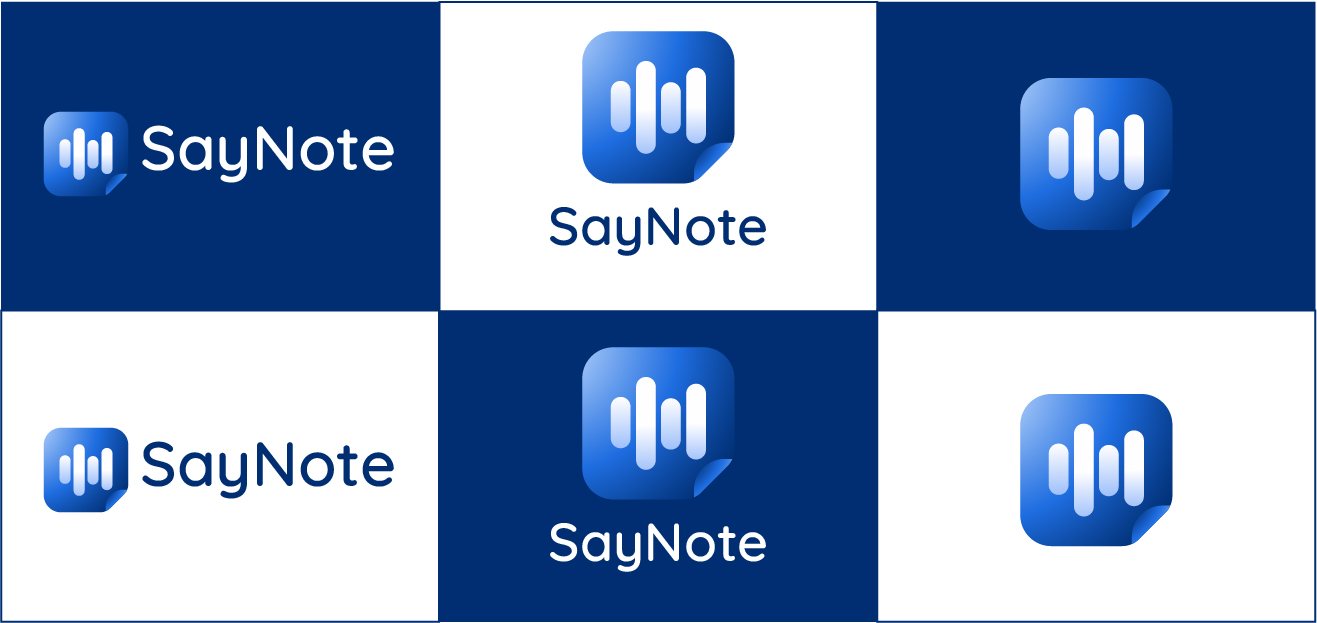
\includegraphics[width=0.7\textwidth]{docs/visual-indentity/pictures/logo-varaition-blue.jpg}
    \caption{Variante bleu du logo. \newline\textit{Cette version met en avant la modernité et la fraîcheur de la marque.}}
\end{figure}

% Explication brève avant chaque figure
\noindent
\textit{La figure suivante illustre un élément clé de l'identité visuelle ou de la communication de la marque.}
\begin{figure}[H]
    \centering
    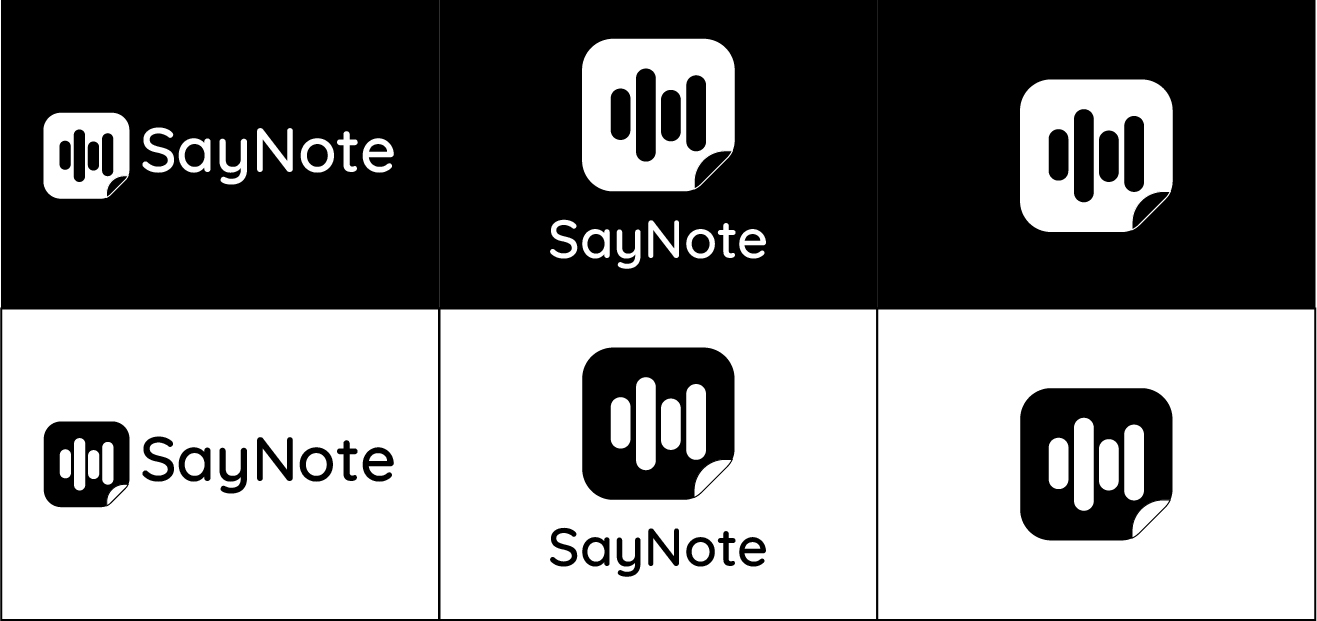
\includegraphics[width=0.7\textwidth]{docs/visual-indentity/pictures/logo-variation-black-and-white.jpg}
    \caption{Logo noir et blanc. \newline\textit{Cette variante assure la lisibilité et l'adaptabilité sur différents supports.}}
\end{figure}

\section{Typographie}
Les polices sans empattement constituent un élément clé de l’identité visuelle de SayNote. Ce choix traduit notre volonté d’offrir une esthétique moderne, épurée et conviviale.

\textbf{a) Police pour les titres}
La police principale d’affichage se distingue par un design géométrique et affirmé, apportant clarté et structure aux titres et messages clés. Ses lignes minimalistes et proportions équilibrées la rendent idéale pour les titres, slogans et zones nécessitant un fort impact visuel.

\textbf{b) Police de contenu}
La police de texte principale est chaleureuse, accueillante et hautement lisible sur tous supports. Ses formes arrondies et son flux harmonieux insufflent une sensation de calme et de proximité à la marque. Elle garantit une excellente lisibilité, même en petite taille, et s’adapte parfaitement aux textes courants, éléments d’interface et contenus étendus.

Ensemble, ces deux polices créent un équilibre harmonieux entre structure et douceur, parfaitement aligné avec l’identité vocale, claire et joyeuse de SayNote.

% Explication brève avant chaque figure
\noindent
\textit{La figure suivante illustre un élément clé de l'identité visuelle ou de la communication de la marque.}
\begin{figure}[H]
    \centering
    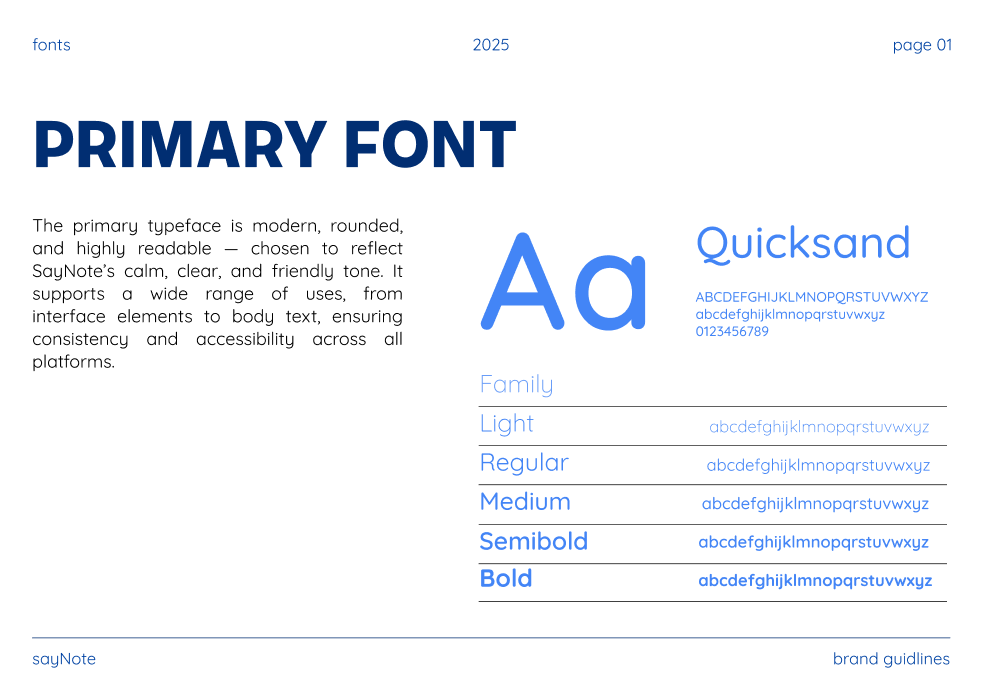
\includegraphics[width=0.7\textwidth]{docs/visual-indentity/pictures/primary-font.png}
    \caption{Police principale SayNote : structure et impact pour les titres. \newline\textit{Cette police renforce la clarté et la hiérarchie visuelle des contenus.}}
\end{figure}
% Explication brève avant chaque figure
\noindent
\textit{La figure suivante illustre un élément clé de l'identité visuelle ou de la communication de la marque.}
\begin{figure}[H]
    \centering
    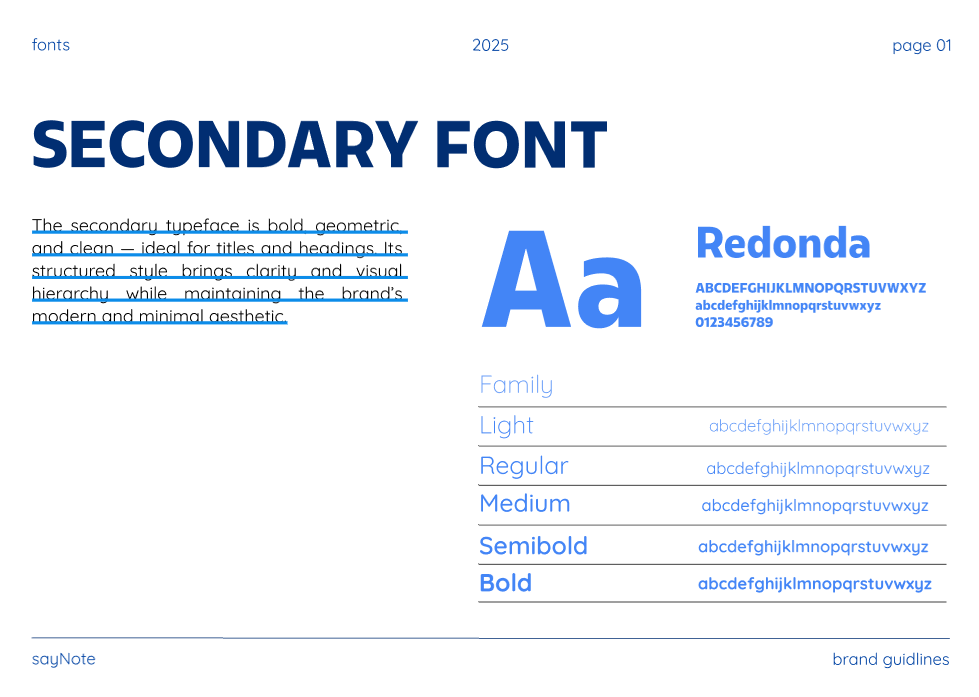
\includegraphics[width=0.7\textwidth]{docs/visual-indentity/pictures/secondery-font.png}
    \caption{Police de contenu SayNote : lisibilité, chaleur et modernité. \newline\textit{Ce choix garantit une lecture agréable et une identité chaleureuse.}}
\end{figure}

\textbf{Titres~:}
Police sans-serif, géométrique, épaisse, pour la clarté et la structure.

\textbf{Corps de texte~:}
Police sans-serif, arrondie et chaleureuse, pour la lisibilité et l’accessibilité.

L’association des deux polices crée un équilibre entre structure et douceur, fidèle à l’esprit SayNote.

\section{Palette de couleurs}
\subsection{Bleu principal — \#4385F6}
Ce bleu vibrant représente la clarté, la confiance et un design intelligent. Il évoque le calme du ciel et la fiabilité des outils numériques modernes. Élément central de l’identité SayNote, il symbolise la concentration, la productivité et la confiance, en parfaite adéquation avec notre objectif d’une expérience vocale sans distraction.

\subsection{Bleus profonds — \#1E6DE0, \#0043A5, \#002E72}
Ces nuances plus sombres complètent la couleur principale en ajoutant profondeur et contraste. Elles reflètent la structure et la clarté de l’interface SayNote, renforçant la stabilité, la précision et une sensation de contrôle calme.

\subsection{Accent clair — \#CFE3FF}
Cet accent pastel doux apporte une touche de légèreté et de joie à l’ensemble de la marque. Il confère une qualité rafraîchissante et aérée à l’interface tout en améliorant la hiérarchie visuelle et l’accessibilité. Il soutient notre ton de clarté et de sérénité, équilibrant les bleus plus soutenus.

% Explication brève avant chaque figure
\noindent
\textit{La figure suivante illustre un élément clé de l'identité visuelle ou de la communication de la marque.}
\begin{figure}[H]
    \centering
    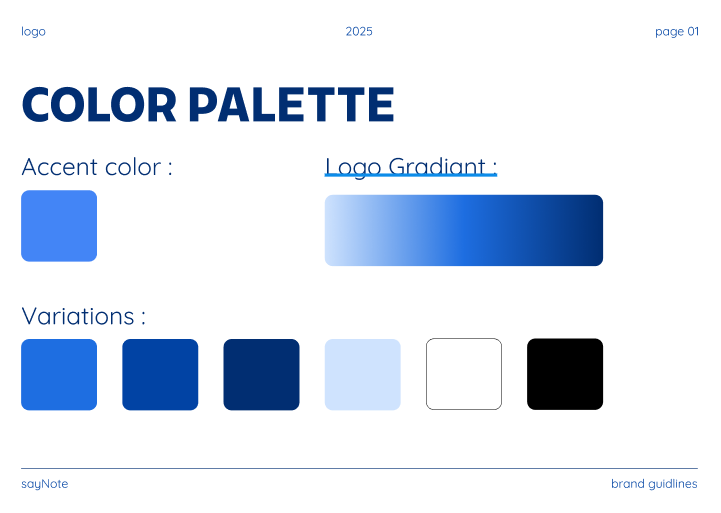
\includegraphics[width=0.6\textwidth]{docs/visual-indentity/pictures/color-palette.png}
    \caption{Palette de couleurs SayNote : harmonie, clarté et confiance.}
\end{figure}

En combinant ces couleurs, SayNote propose un système visuel harmonieux et émotionnellement aligné, reflétant nos valeurs fondamentales : clarté, confiance, inclusivité et productivité sereine.

\section{Stationery \& Visual Imagination}
\subsection{Design}
La papeterie SayNote comprend une gamme complète de supports imprimés, conçus pour refléter l'identité visuelle de la marque et renforcer la cohérence graphique dans toutes les communications professionnelles.

\subsubsection*{Carte de visite}
La carte de visite SayNote reprend les codes graphiques de la marque : couleurs, typographie et logo. Elle offre une présentation professionnelle et mémorable lors des échanges.
% Explication brève avant chaque figure
\noindent
\textit{La figure suivante illustre un élément clé de l'identité visuelle ou de la communication de la marque.}
\begin{figure}[H]
    \centering
    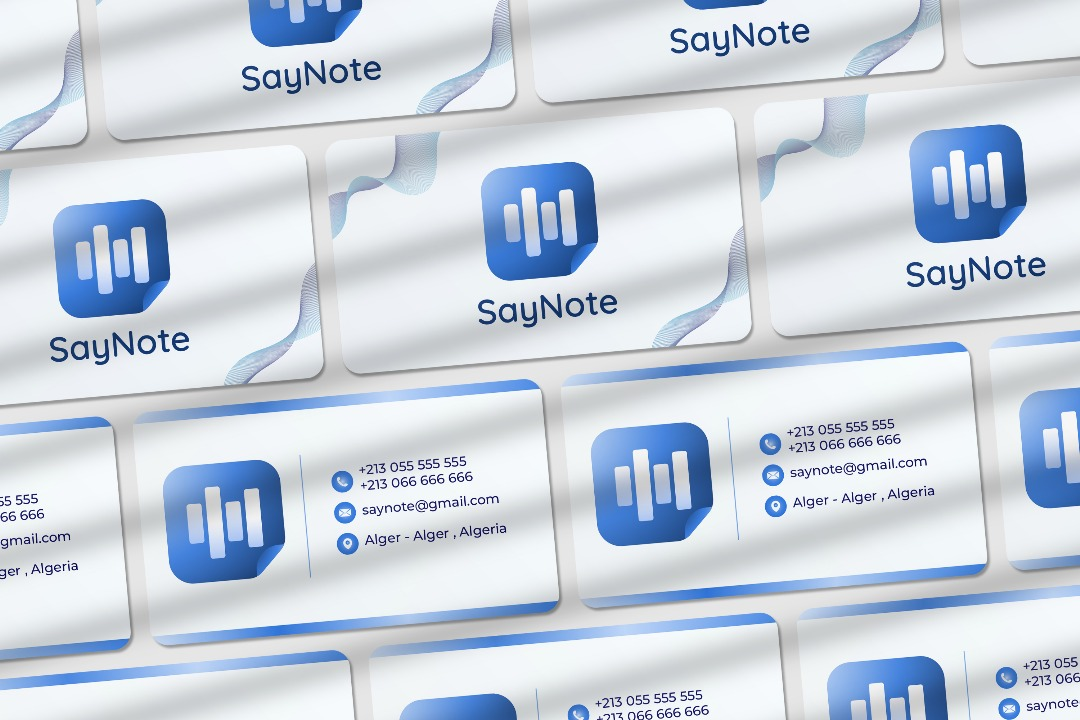
\includegraphics[width=0.5\textwidth]{docs/visual-indentity/pictures/card.jpg}
    \caption{Carte de visite SayNote : design épuré et impactant. \newline\textit{Un support professionnel qui véhicule l'identité de la marque.}}
\end{figure}

\subsection{Poster}
\subsubsection*{a) Concept du design}
Le concept du poster repose sur l'attraction visuelle, l'expression de l'identité de la marque et la mise en avant des fonctionnalités clés de SayNote. La composition soigneusement pensée allie des images frappantes, des couleurs vibrantes de la marque et un texte concis et percutant pour assurer lisibilité et impact. Les posters finaux sont conçus au format A3.

\subsubsection*{b) Versions}
Deux versions de posters ont été réalisées pour répondre à différents usages et publics. La première met l’accent sur la productivité vocale de SayNote, tandis que la seconde valorise la clarté et la fluidité apportées par l’IA et le design. Les deux affiches conservent une cohérence visuelle tout en ciblant des besoins et contextes variés.

\subsubsection*{c) Développement du contenu}
Le contenu a été élaboré pour délivrer un message convaincant : titres accrocheurs, valeurs essentielles et un appel à l’action clair (téléchargement de l’application ou visite du site). Les visuels et le texte reflètent le ton de la marque : calme, clarté, soutien et modernité.

% Explication brève avant chaque figure
\noindent
\textit{La figure suivante illustre un élément clé de l'identité visuelle ou de la communication de la marque.}
\begin{figure}[H]
    \centering
    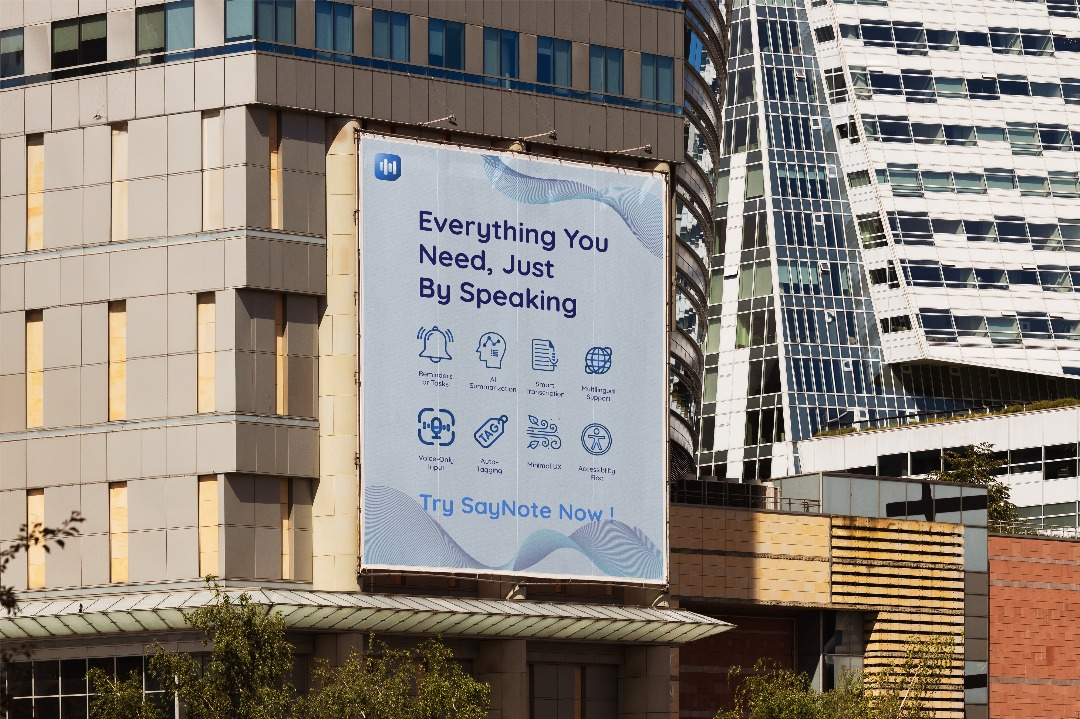
\includegraphics[width=0.8\textwidth]{docs/visual-indentity/pictures/poster2.jpg}
    \caption{Poster SayNote : version "Productivité Vocale" – met en avant la rapidité et la simplicité de la prise de notes par la voix. \newline\textit{Ce poster valorise l'usage vocal et la modernité de l'application.}}
\end{figure}
% Explication brève avant chaque figure
\noindent
\textit{La figure suivante illustre un élément clé de l'identité visuelle ou de la communication de la marque.}
\begin{figure}[H]
    \centering
    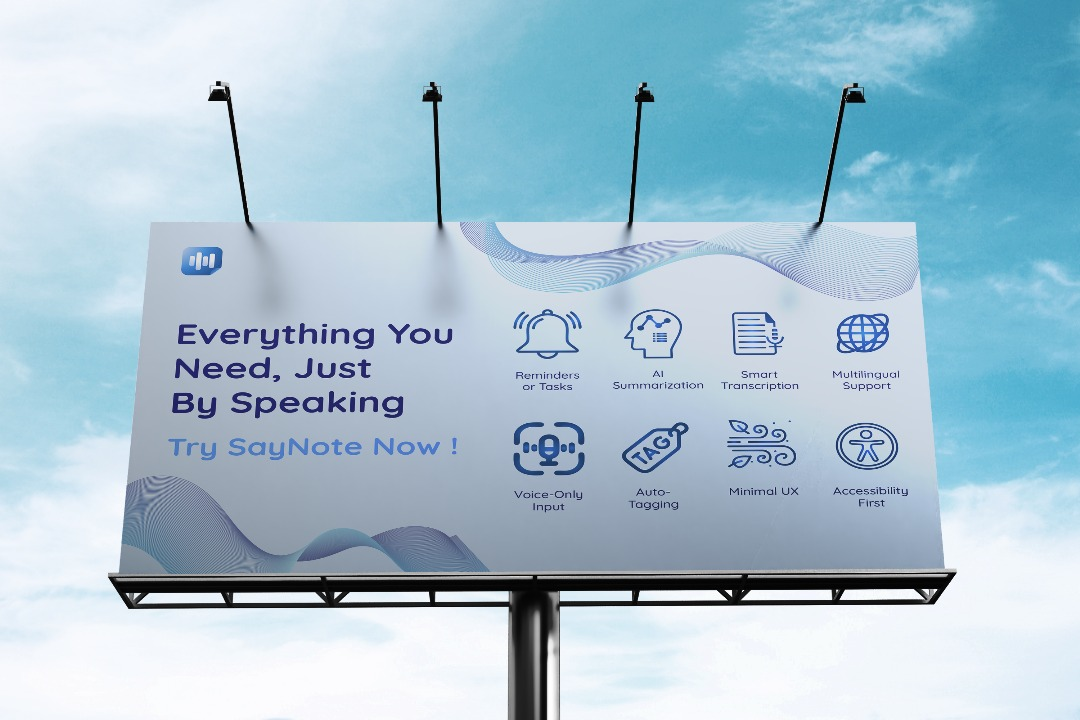
\includegraphics[width=0.8\textwidth]{docs/visual-indentity/pictures/poster.jpg}
    \caption{Poster SayNote : version "Clarté et Innovation" – valorise la fluidité, la technologie et le design moderne de l’application.}
\end{figure}

\subsection{Banner}
\subsubsection*{a) Concept du design}
La bannière SayNote est conçue pour renforcer la présence visuelle de la marque lors d’événements ou dans des espaces digitaux. Elle s’appuie sur une composition graphique forte, des couleurs distinctives et des éléments identitaires pour attirer l’attention et transmettre les valeurs du projet.

\subsubsection*{b) Développement du contenu}
Les messages mis en avant sur la bannière sont pensés pour promouvoir la crédibilité, la modernité et la cohérence de la marque, tout en assurant une lisibilité optimale à distance. Les éléments graphiques sont harmonisés avec l’ensemble de la papeterie et des supports visuels.

\subsubsection*{c) Éléments visuels}
% Explication brève avant chaque figure
\noindent
\textit{La figure suivante illustre un élément clé de l'identité visuelle ou de la communication de la marque.}
\begin{figure}[H]
    \centering
    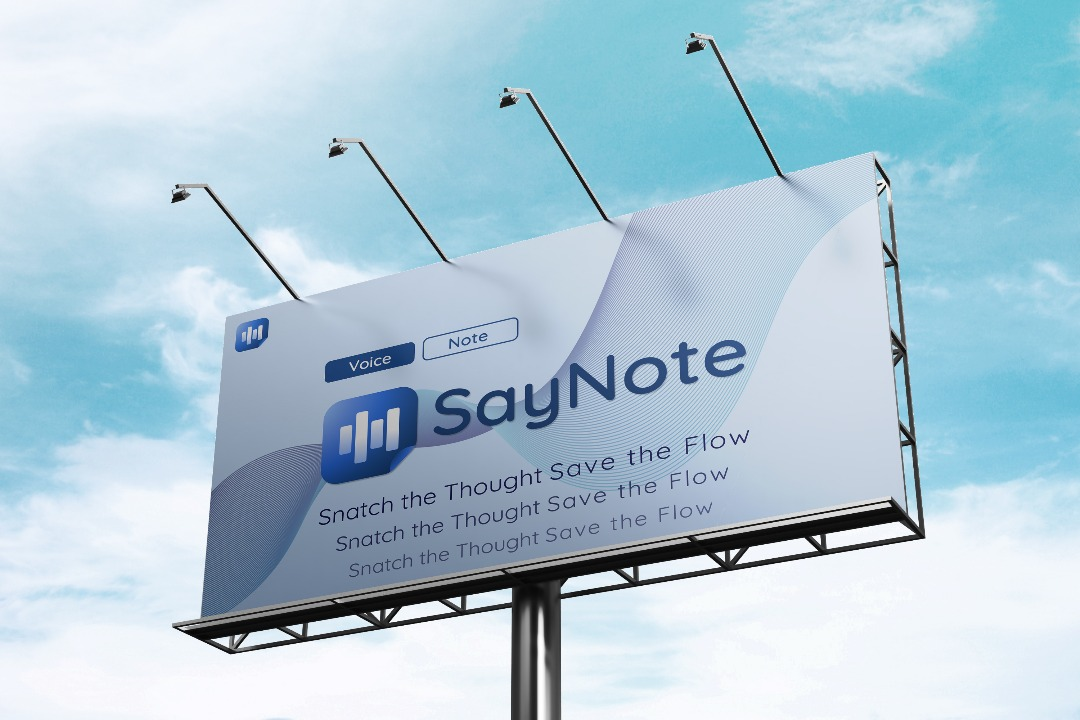
\includegraphics[width=0.8\textwidth]{docs/visual-indentity/pictures/big-banner.jpg}
    \caption{Bannière principale SayNote : composition graphique forte et identité affirmée. \newline\textit{La bannière incarne la présence visuelle de la marque lors d'événements et en ligne.}}
\end{figure}
% Explication brève avant chaque figure
\noindent
\textit{La figure suivante illustre un élément clé de l'identité visuelle ou de la communication de la marque.}
\begin{figure}[H]
    \centering
    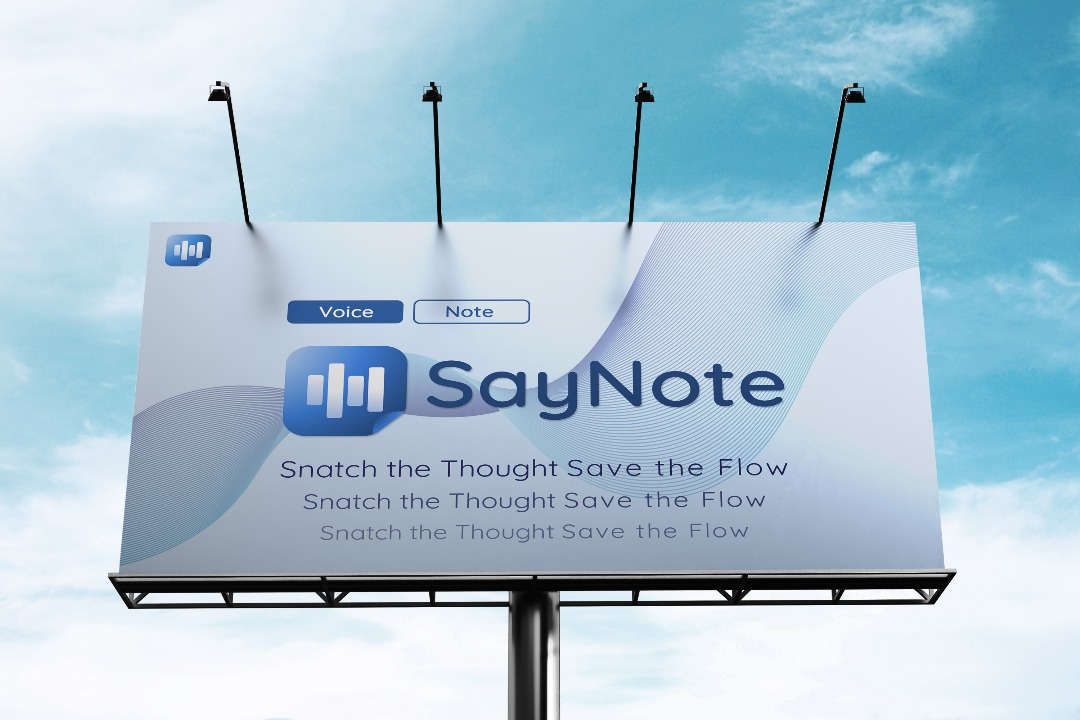
\includegraphics[width=0.8\textwidth]{docs/visual-indentity/pictures/big-banner-directly .jpg}
    \caption{Variante directe de la bannière SayNote : adaptation pour différents contextes visuels. \newline\textit{Cette déclinaison assure la flexibilité de la marque sur divers supports.}}
\end{figure}

\subsection{Flyer (Brochure)}
\subsubsection*{a) Concept du design}
Le flyer SayNote reprend l’ensemble de l’identité visuelle de la marque pour offrir un support de communication synthétique, élégant et professionnel. Il met en avant la cohérence graphique et la qualité des supports imprimés.

\subsubsection*{b) Développement du contenu}
Le contenu du flyer est pensé pour présenter les atouts de la marque et renforcer la reconnaissance auprès du public cible. La sélection d’images illustre la diversité et la qualité des supports :

% Explication brève avant chaque figure
\noindent
\textit{La figure suivante illustre un élément clé de l'identité visuelle ou de la communication de la marque.}
\begin{figure}[H]
    \centering
    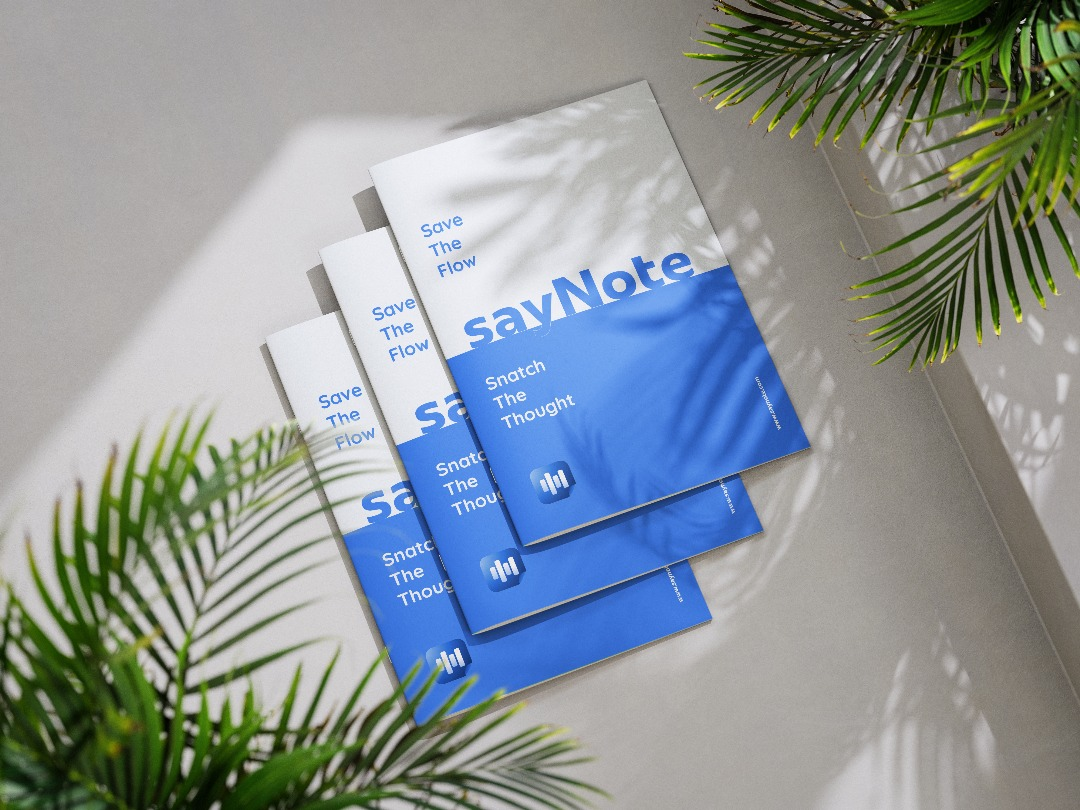
\includegraphics[width=0.7\textwidth]{docs/visual-indentity/pictures/pappiers.jpg}
    \caption{Aperçu général de la papeterie SayNote : enveloppes, blocs-notes et feuilles personnalisées.}
\end{figure}
% Explication brève avant chaque figure
\noindent
\textit{La figure suivante illustre un élément clé de l'identité visuelle ou de la communication de la marque.}
\begin{figure}[H]
    \centering
    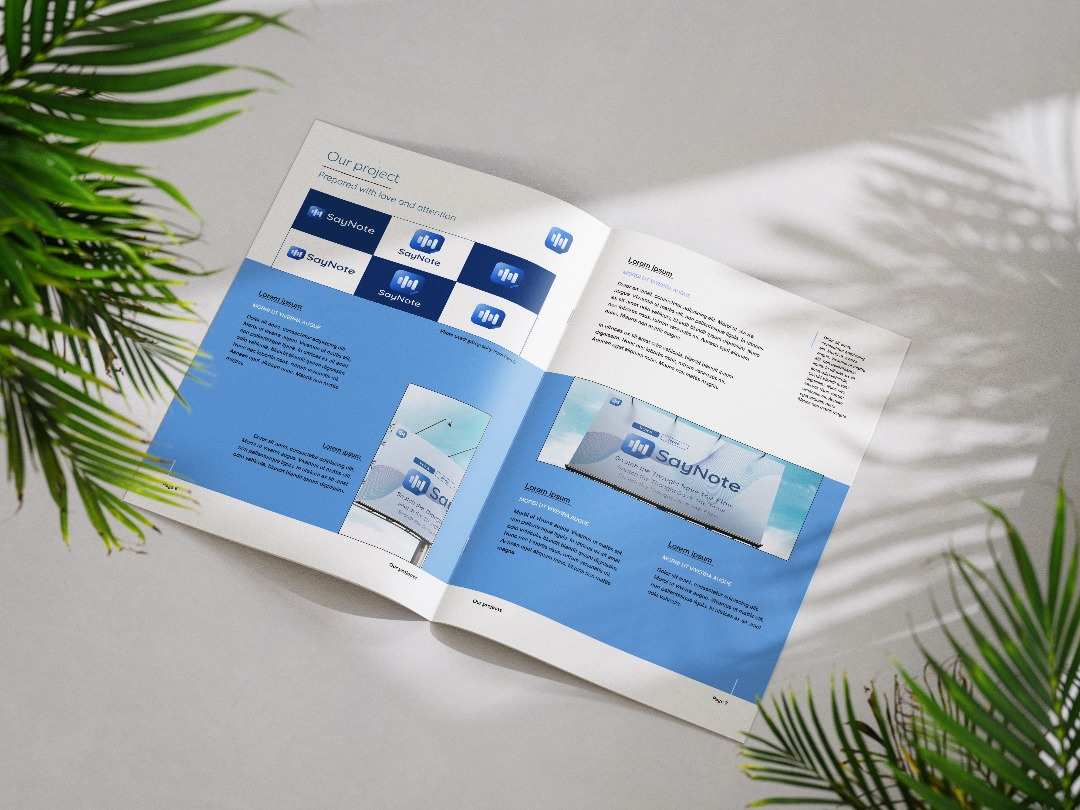
\includegraphics[width=0.7\textwidth]{docs/visual-indentity/pictures/pappier.jpg}
    \caption{Papier à en-tête SayNote : design épuré et professionnel. \newline\textit{Un élément essentiel de la papeterie qui renforce la cohérence de l'identité graphique.}}
\end{figure}
% Explication brève avant chaque figure
\noindent
\textit{La figure suivante illustre un élément clé de l'identité visuelle ou de la communication de la marque.}
\begin{figure}[H]
    \centering
    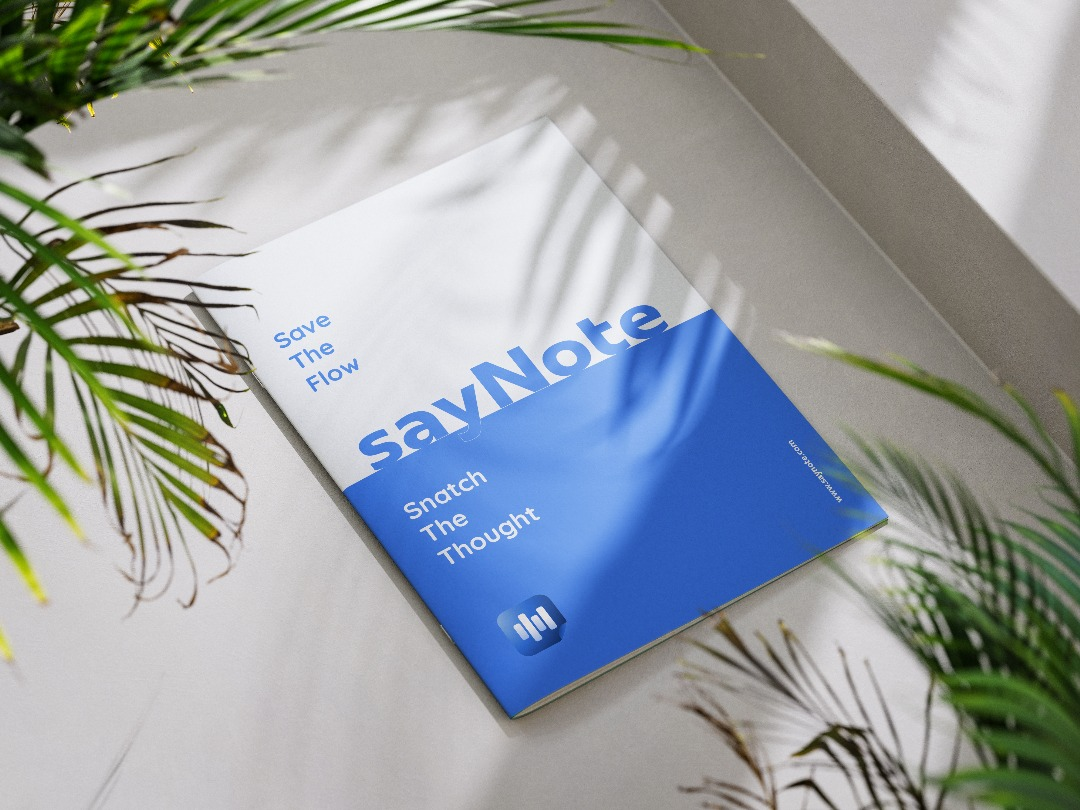
\includegraphics[width=0.7\textwidth]{docs/visual-indentity/pictures/pappier-back.jpg}
    \caption{Verso du papier à en-tête SayNote : souci du détail et harmonie visuelle. \newline\textit{Le verso complète l'expérience de marque jusque dans les moindres détails.}}
\end{figure}



\section{Conclusion}
La création d'une identité de marque est un processus dynamique et itératif qui nécessite une planification minutieuse, de la créativité et une attention aux détails. C'est un voyage continu de perfectionnement et de renforcement de l'identité de la marque afin d'assurer cohérence et pertinence dans un marché en constante évolution. Grâce à un positionnement stratégique, un design visuel, des messages convaincants et une expérience de marque cohérente, les organisations peuvent se différencier de leurs concurrents, établir un lien émotionnel fort avec leur public et favoriser la fidélité à la marque. En investissant du temps et des efforts dans le processus de création de l'identité de marque, les entreprises peuvent poser des bases solides pour un succès à long terme, leur permettant de communiquer efficacement leurs valeurs, de tenir leurs promesses et de laisser une impression durable dans l'esprit des consommateurs. En fin de compte, une identité de marque bien définie devient un atout puissant qui aide les entreprises à prospérer et à avoir un impact significatif dans leurs secteurs respectifs.

% --- Conclusion non numérotée ---
\vspace{1cm}
\begin{center}
\end{center}



\section*{Conclusion}
\addcontentsline{toc}{section}{Conclusion}
Ce chapitre a mis en lumière l'importance d'une conception réfléchie, de la planification à l'identité visuelle. L'intégration de l'UX et du branding garantit une expérience utilisateur optimale et une marque forte, éléments essentiels pour le succès et la différenciation du projet SayNote.
